\documentclass[11pt,oneside,a4paper]{book}
% \usepackage[a5paper]{geometry}
\usepackage[utf8]{inputenc}
\usepackage[czech, english]{babel}
\usepackage{listings}
\usepackage{algorithmic}
\usepackage{todonotes}
\usepackage{graphicx}
\usepackage{natbib}
\usepackage{amsthm}
\usepackage{subfig}
\usepackage{rotating}
\usepackage{epigraph}
\usepackage{framed}
\usepackage{url}
\usepackage{tabulary}
\usepackage{float}
\usepackage{mdwlist}
\usepackage{multirow}
\usepackage[helvetica]{quotchap}
% \usepackage{times}
\usepackage{graphviz}

\newcommand{\myepigraph}[2]{\begin{savequote}[10pc]\sffamily #1 \qauthor{#2}\end{savequote}}
\renewcommand\chapterheadstartvskip{\vspace*{-4\baselineskip}}

\interfootnotelinepenalty=10000
	
\theoremstyle{definition}
\newtheorem{definition}{Definition}

% \setlength{\epigraphrule}{0pt}

\lstdefinelanguage{CSharp}
{
 morecomment = [l]{//}, 
 morecomment = [l]{///},
 morecomment = [s]{/*}{*/},
 morestring=[b]", 
 sensitive = true,
 morekeywords = {abstract,  event,  new,  struct,
   as,  explicit,  null,  switch,
   base,  extern,  object,  this,
   bool,  false,  operator,  throw,
   break,  finally,  out,  true,
   byte,  fixed,  override,  try,
   case,  float,  params,  typeof,
   catch,  for,  private,  uint,
   char,  foreach,  protected,  ulong,
   checked,  goto,  public,  unchecked,
   class,  if,  readonly,  unsafe,
   const,  implicit,  ref,  ushort,
   continue,  in,  return,  using,
   decimal,  int,  sbyte,  virtual,
   default,  interface,  sealed,  volatile,
   delegate,  internal,  short,  void,
   do,  is,  sizeof,  while,
   double,  lock,  stackalloc,   
   else,  long,  static,   
   enum,  namespace,  string}
}

 \lstset{
         basicstyle=\footnotesize\ttfamily, % Standardschrift
         commentstyle=\color[HTML]{008000},
         %numbers=left,               % Ort der Zeilennummern
         numberstyle=\tiny,          % Stil der Zeilennummern
         %stepnumber=2,               % Abstand zwischen den Zeilennummern
         numbersep=5pt,              % Abstand der Nummern zum Text
         tabsize=2,                  % Groesse von Tabs
         extendedchars=true,         %
         breaklines=true,            % Zeilen werden Umgebrochen
         keywordstyle=\color{blue},
    		frame=b,         
 %        keywordstyle=[1]\textbf,    % Stil der Keywords
 %        keywordstyle=[2]\textbf,    %
 %        keywordstyle=[3]\textbf,    %
 %        keywordstyle=[4]\textbf,   \sqrt{\sqrt{}} %
         stringstyle=\color{white}\ttfamily, % Farbe der String
         showspaces=false,           % Leerzeichen anzeigen ?
         showtabs=false,             % Tabs anzeigen ?
         xleftmargin=17pt,
         framexleftmargin=17pt,
         framexrightmargin=5pt,
         framexbottommargin=4pt,
         %backgroundcolor=\color{lightgray},
	columns=flexible,
         showstringspaces=false      % Leerzeichen in Strings anzeigen ?        
 }
\DeclareCaptionFont{white}{\color{white}}
\DeclareCaptionFormat{listing}{\colorbox[cmyk]{0.43, 0.35, 0.35,0.01}{\parbox{\textwidth}{\hspace{13pt}#1#2#3}}}
\captionsetup[lstlisting]{format=listing,labelfont=white,textfont=white,singlelinecheck=false,margin=0pt,font={bf,footnotesize}}

\makeatletter
\newcommand\fs@plainruled{\def\@fs@cfont{\bfseries}\let\@fs@capt\floatc@ruled
  \def\@fs@pre{\kern2pt}%
  \def\@fs@post{\kern2pt\hrule\relax}%
  \def\@fs@mid{\kern2pt}%
  \let\@fs@iftopcapt\iftrue}
\makeatother

\floatstyle{plainruled}
\newfloat{myalgorithm}{htbp}{loa}
\floatname{myalgorithm}{Algorithm}
\captionsetup[myalgorithm]{format=listing,labelfont=white,textfont=white, singlelinecheck=false, margin=0pt, font={bf,footnotesize}}

\hyphenation{SymbolicObject SymbolicObjects}

\mathchardef\mhyphen="2D

\makeatletter
\begingroup
  \catcode`\-=\active
  \def\x{\endgroup
  \let\cs@cline\@cline
  \expandafter\def\expandafter\@cline
    \expandafter##\expandafter1\expandafter
      -\expandafter##\expandafter2\expandafter\@nil\expandafter
        {\expandafter\cs@cline\expandafter##\expandafter1\minus##2\@nil}
}\x
\makeatother

\begin{document}
%\maketitle

\pagestyle{plain}\pagenumbering{roman}
\selectlanguage{english}

\begin{titlepage}
\cleardoublepage
\thispagestyle{empty}
\begin{center}
\large\rmfamily
Czech Technical University in Prague\\
Faculty of Electrical Engineering\\
Department of Cybernetics\\
\vglue 10mm

\includegraphics[width=50mm]{LogoCVUT}
\vglue 30mm
{\large Diploma Thesis}\\
\bigskip
{\Large\bf Finding Deadlocks Using Static Code Analysis}\\
\bigskip
\bigskip
{\Large\it Filip Navara}\\
\vfill
\item[Supervisor:]\ Ing. Radek Mařík, CSc.\\
\vglue 15mm
{Study Programme: Open Informatics}\\
\bigskip
{Field of Study: Computer Engineering}\\
\bigskip
\today
\end{center}
\end{titlepage} 
\cleardoublepage
\vspace*{\fill}
\noindent
{\huge {%
Acknowledgements%
}}
\vspace{3ex}\par

In 2008, when I was still studying at Czech Technical University for a bachelor's degree I attended a Theorical Computer Science course with Mgr. Petr Matyáš. He taught me basics of graph theory, which served important role in my reasoning about mathematical and computer science problems. My final work for the course served as a basis for this thesis. It was a home work written over the course of single weekend, which targeted the same goals as this thesis. Unfortunately at that time my understanding of the problem was very limited, yet the work has taught me that I wasn't aiming for an impossible target.

A year later, in 2009, Ing. Ladislav Vagner, Ph.D. thought me the basics of compiler construction and intermediate representation of computer programs. This provided me with the necessary theoretical background for understanding how optimizing compilers work, which is very close to how static code analysis tools work.

In 2011, I attended a Software Verification and Testing class with Ing. Radek Mařík, CSc. The class provided me with deeper understanding of how programs can be analyzed and renewed my interest in the static code analysis. It also introduced me to model checkers and their ability to detect deadlocks. He later became my supervisor for this thesis and only thanks to his dedication and experience I was able to finish all the work in time.

Lastly, and most importantly, I wish to thank my family for supporting me throughout all my studies. 
\cleardoublepage
\vspace*{\fill}
\noindent
{\huge {%
Declaration%
}}
\vspace{3ex}\par
\noindent
\noindent
I hereby declare that I have completed this thesis independently and that I have listed all the literature and publications used.\\
I have no objection to usage of this work in compliance with the act \S 60 Zákon č.~121/2000Sb. (copyright law), and with the rights connected with the copyright act including the changes in the act.%
\\[15mm]
Prague, \today \hfill \hbox to 70mm{\tiny\dotfill}

\cleardoublepage
\noindent
%{\Huge \textbf{Abstract}}
%\vspace{8ex}
\chapter*{Abstract}

The thesis explores an algorithm for finding potential deadlocks in parallel programs written for the .NET Framework. Our goal is to simplify testing of parallel programs and to determine places in the code that could possibly cause problems and that should be examined as a part of the software testing life cycle.

We present a design and implementation of an algorithm for finding these potential deadlock possibilities by construction of a lock-order graph by a static code analysis. This graph represents the order in which locks are acquired by the program. Cycles in the graph indicate deadlock possibilities, and our tool reports them.

We evaluated the implementation on one commercial application and identified that 4 out of the 40 reported possibilities may lead to a deadlock. 

\vglue60mm

\begin{flushright}
{\noindent{\huge {Abstrakt}}}
\vskip 2.75\baselineskip
\end{flushright}

{\selectlanguage{czech}
\noindent
Tato práce zkoumá algoritmus pro hledání potenciálních uváznutí v paralelních programech napsaných pro .NET Framework. Našim cílém je usnadnění testování paralelních programů a nalezení míst v kódu, kde by potenciálně mohlo dojít k uváznutí, aby mohla tato místa být prozkoumána v rámci životního cyklu testování softwaru.

Představujeme návrh a implementaci algoritmu pro nalezení potenciálních uváznutí pomocí sestrojení lock-order grafu statickou analýzou kódu. Tento graf reprezenuje pořadí, v němž jsou zámky programem uzamykány. Smyčky v tomto grafu reprezentují možná uváznutí a náš nástroj tato možná uváznutí vypisuje.

Implementaci jsme vyhodnotili spuštěním na komerční aplikaci, kde jsme ověřili, že z 40 vypsaných možností uváznutí vedou 4 na skutečná uváznutí v programu.
}

\setcounter{tocdepth}{1}
\tableofcontents

\cleardoublepage
\pagestyle{headings}\pagenumbering{arabic}\setcounter{page}{1}

\myepigraph{Irreproducible bugs become highly reproducible right after delivery to the customer.}%
         {Michael Stahl}
\chapter{Introduction}

\section{Motivation}

Modern software design includes concurrent programming. It is widely accepted that designing and testing concurrent programs is hard. Two major problems with designing concurrent programs are deadlocks and race conditions.

Deadlock is a condition under which program is halted because each thread in a set is waiting for a resource that is currently held by other thread in the set. Since deadlocks prevent the application from running, it poses a significant problem.

Finding deadlocks using traditional testing techniques, such as unit tests, integration tests and validation testing, proved to be difficult since reaching a deadlock may require a specific interleaving of threads. It is usually infeasible to simulate all thread interleavings of a program, because it has exponential complexity with regard to the number of threads.

Many techniques \citep{Hewitt1973} and language extensions \citep{Agarwal2006,Permandla2007} were developed that aim to reduce or eliminate the potential for deadlocks at the expense of requiring the programmer to learn new methods of how to write programs. This approach has two major drawbacks. Firstly, the learning curve is often very steep and thus the programmer has to spend more time to learn the new techniques. Secondly, there are often large legacy code bases that can't be easily refactored to accompany the new techniques. These drawbacks largely contribute to the fact that these techniques are rarely used outside of the academic community and mission critical systems.

\section{Objectives}

This paper aims at introducing a design of a tool for analyzing whole programs written for the .NET Framework for a potential presence of deadlocks in the code.

The tool will operate on programs without actually executing them using a set of techniques known as static program analysis. Benefit of this approach is that the tool can readily be run on existing programs with no modifications required. It will work on legacy code bases and require no changes to the design of  programs or language.

A reference implementation of the design will be provided and evaluated on several test programs and one commercial application.

The objective is to provide a tool that is fast enough to be used on large scale code bases. At the same time the amount of false positives reported by the tool should be minimized to allow for manual inspection of the results.  

\section{Overview}

The rest of the paper is organized as follows. In Chapter 2 an overview of .NET Framework and its locking mechanisms is given, followed by explanation of how the mechanisms can lead to deadlock. In Chapter 3, we provide a brief introduction to static program analysis techniques. Chapter 4 gives an overview of existing methods and tools for deadlock detection. In Chapter 5 a design is outlined for the analysis. Chapter 6 describes the architecture of the tool and implementation details. In Chapter 7, we present experimental results. Finally, we describe the future work in Chapter 8.

\myepigraph{When two trains approach each other at a crossing, both shall come to a full stop and neither shall start up again until the other has gone.}%
         {Kansas State Law, early 20th century}
\chapter{Background}

In this chapter we will describe what .NET Framework is, which locking mechanisms are available in the framework and how usage of these locking mechanisms can lead to deadlock. We will also introduce lock order graph structure that is used by many of deadlock detection tools, which are described later in Chapter 4.

\section{.NET Framework}

The .NET Framework is a general-purpose software development platform similar to the Java Development Kit. It includes a rich class library (Base Class Library or BCL) and a virtual machine model that is independent of the underlying platform.

The platform independent code is stored using an intermediate language (also referred to as Common Intermediate Language, CIL, IL or bytecode). The data are passed around between individual instructions using a stack. The instructions are aware of the object-oriented programming model and are more high-level than the native processor instructions. For example, there are instructions to allocate a new object, load a field from object or to call a virtual method.

Information about the program structure is largely preserved in metadata of the executable files. This includes class structure, typing information and method signatures. The code also remains separated into individual methods.

The virtual machine is intended to be type-safe and verifies the code before execution. However, the .NET Framework also supports a notion of unsafe code that operates on pointers. The unsafe code is most commonly used for interoperability with native platform libraries and its use makes the program unverifiable. The virtual machine may disallow execution of unsafe code based on the security context the application is run under.

Unlike Java, the .NET intermediate language has notion of generics, function pointers (called \emph{delegates}) and passing of parameters by reference.

A more detailed overview of the .NET framework is given in ECMA-335 standard \citep{Ecma335}.

\section{Locks in .NET Framework}

In .NET Framework, each object has an associated lock. This lock can be acquired using the \texttt{Monitor.Enter} or \texttt{Monitor.TryEnter} method and released using the \texttt{Monitor.Exit} method. The C\# language also offers a simplified \texttt{lock (object)} construct that is translated by the compiler to appropriate \texttt{Monitor.Enter} and \texttt{Monitor.Exit} calls with proper exception handling (Listing ~\ref{fig:lock20} and ~\ref{fig:lock40}). While not enforced by the runtime it is an accepted practice, supported by the language syntax, that locks are released in reverse order of their acquisition.

A lock that is held by one thread cannot be acquired in another thread until the first thread releases it. Thread blocks if an attempt is made to acquire lock that is held by another thread and it is blocked until it successfully acquires the lock\footnote{The thread may not be completely blocked. Due to compatibility with COM, a thread that uses single thread apartment model has to process incoming messages while waiting for the lock to be acquired. This is implemented internally using the \texttt{SynchronizationContext} abstraction and the \texttt{CoWaitForMultipleObjects} Win32 API function. It may cause unexpected changes to the lock hierarchy for implementations of COM objects and for paint messages in UI frameworks such as WPF and System.Windows.Forms.}. Exception to this behavior is the \texttt{Monitor.TryEnter} method which allows execution to continue even if the lock wasn't acquired provided that a specified timeout was reached while waiting for the lock to be released by another thread.

Locks are held per-thread and they are re-entrant. Acquiring a lock that is already held by the thread doesn't block the execution and the lock is released when the outermost \texttt{Monitor.Exit} for the given lock is called.

Methods \texttt{Monitor.Wait}, \texttt{Monitor.Pulse} and \texttt{Monitor.PulseAll} are available to facilitate signaling. All of these methods operate on locks that are already held.

When a thread calls \texttt{Monitor.Wait}, it releases the lock on the object and enters the object's waiting queue. The next thread in the object's ready queue (if there is one) acquires the lock and has exclusive rights to the object. All threads that call \texttt{Monitor.Wait} remain in the waiting queue until they receive a signal from \texttt{Monitor.Pulse} or \texttt{Monitor.PulseAll}. Once a thread is removed from an object's waiting queue, the \texttt{Monitor.Wait} method attempts to reacquire the lock for the object it was invoked on. The method returns only after the lock is reacquired.

The .NET Framework also offers other locking primitives, such as \texttt{Mutex}, \texttt{AutoResetEvent}, \texttt{ManualResetEvent} and \texttt{Semaphore}, that offer different capabilities than the regular locks. These locking primitives are implemented using operating system kernel objects and thus they can be used for inter-process synchronization. Semantics of these locking primitives also differ from regular locks in terms of reentrancy and thread ownership.

For a more detailed overview of threading and locking mechanisms in .NET Framework please refer to the Threading in C\# book \citep{Albahari2006}.

\begin{lstlisting}[language=CSharp,caption=lock(o) construct in C\# 2.0,label=fig:lock20]
Monitor.Enter(o);
try
{
   ...
}
finally
{
   Monitor.Exit(o);
}
\end{lstlisting}

\begin{lstlisting}[language=CSharp,caption=lock(o) construct in C\# 4.0,label=fig:lock40]
bool acquired = false;
try
{
   Monitor.Enter(o, ref acquired);
   ...
}
finally
{
   if (acquired)
      Monitor.Exit(o);
}
\end{lstlisting}

\section{Deadlock}

For a deadlock to occur it is necessary to fulfill a set of conditions known as \emph{Coffman conditions} \citep{Coffman1971}. The necessary conditions are the following:
\begin{itemize*}
\item \emph{mutual exclusion} - Tasks claim exclusive control of a resource they require.
\item \emph{hold and wait} - Tasks hold resources that already have control of while waiting to acquire additional resources.
\item \emph{no preemption} - Resources are not forcibly removed from under the task that currently controls them. The task is responsible for releasing the resource it acquired.
\item \emph{circular wait} - Two or more tasks form a circular chain where each task waits for a resource already owned by a different task in the set.
\end{itemize*}

In .NET, the tasks can be seen as threads and the resources as the implicit locks associated with every object. It is possible to hit all four conditions in .NET and thus deadlock can occur. 

The circular wait condition itself is very broadly defined and can further be dissected into subconditions that have to be met for the deadlock to occur:
\begin{itemize*}
\item \emph{Lock order inversion} - Locks on two or more objects are acquired in different code paths in different order (Listing ~\ref{fig:lockOrderInversion2} and ~\ref{fig:lockOrderInversion3}).
\item \emph{Parallel execution} - The lock order inversion has to happen in two separate threads that may run in parallel.
\item \emph{No guard lock} - If each lock order inversion is guarded by an additional lock, also known as \emph{guard lock}, then no execution path can actually reach the locks in inverted order and thus the inversion cannot cause a deadlock (Listing ~\ref{fig:lockOrderInversionGuard}).
\end{itemize*}

\begin{lstlisting}[language=CSharp,caption=Lock order inversion with 2 resources,label=fig:lockOrderInversion2]
/* Thread 1: */ lock (a) { lock (b) { ... } }
/* Thread 2: */ lock (b) { lock (a) { ... } }
\end{lstlisting}

\begin{lstlisting}[language=CSharp,caption=Lock order inversion with 3 resources,label=fig:lockOrderInversion3]
/* Thread 1: */ lock (a) { lock (b) { ... } }
/* Thread 2: */ lock (b) { lock (c) { ... } }
/* Thread 3: */ lock (c) { lock (d) { ... } }
\end{lstlisting}

\begin{lstlisting}[language=CSharp,caption=Lock order inversion protected by guard lock,label=fig:lockOrderInversionGuard]
/* Thread 1: */ lock (c) { lock (a) { lock (b) { ... } } }
/* Thread 2: */ lock (c) { lock (b) { lock (a) { ... } } }
\end{lstlisting}

\section{Lock order graph}

A graph representation of the lock order hierarchy is called \emph{lock order graph}. Each vertex in the graph is a resource that program locks on. Each edge represents a lock hierarchy, ie. acquisition of resource $r_1$ while already holding resource $r_2$ is represented by an edge $r_1 \rightarrow r_2$.

\begin{definition}
A \emph{lock order graph} is directed graph $\langle N, E \rangle$, where $N$ is the set of vertices corresponding to abstract objects that are used as locks, and $E$ is the set of directed edges that reflect the order in which each thread acquires the locks.
\end{definition}

\begin{definition}
Additionally we define a set \emph{roots} that specifies vertices of the lock order graph that are top-level locks in any thread.
\end{definition}

\begin{figure}[h]
\begin{center}
\digraph[scale=0.65]{LockOrderInversion2}{
a -> b;
b -> a;
}
\caption{Lock order inversion with 2 resources}
\end{center}
\end{figure}

\begin{figure}[h]
\begin{center}
\digraph[scale=0.65]{LockOrderInversion3}{
a -> b;
b -> c;
c -> a;
}
\caption{Lock order inversion with 3 resources}
\end{center}
\end{figure}

\begin{figure}[h]
\begin{center}
\digraph[scale=0.65]{LockOrderInversionGuard}{
c -> a;
a -> b;
b -> a;
c -> b;
}
\caption{Lock order inversion protected by guard lock}
\end{center}
\end{figure}

\chapter{Static program analysis}

Static code analysis is a field of computer science that studies algorithms for analyzing the program code. As opposed to dynamic code analysis that relies on executing the code and capturing information during the execution, the static analysis works on code without ever executing it. Techniques studied in this field are leveraged in today's optimizing compilers and specialized tools for verifying program correctness.

It is important to note that according to the Rice's theorem \citep{Rice1953} any non-trivial property of the program behavior in a Turing-complete language is undecidable. Thus most of the techniques outlined below compute only conservative approximate answers. The engineering challenge is to use a correct combination of the algorithms and to choose a correct approximation for a particular problem. Most of the methods outlined below could be implemented with different levels of precision at the cost of the analysis time. While it may be tempting to assume that the most precise method will always give the best answer it was shown before \citep{Milanova2002} that even less precise methods could lead to the best solutions.

The rest of this chapter is organized as follows. Section 3.1 describes the analysis of program metadata and defines class hierarchy graph. Section 3.2 describes the concepts behind intraprocedural analysis, specifically the control-flow graphs and data-flow analysis and shows how to implement them. Section 3.3 then extends the intraprocedural concepts to interprocedural level.

\section{Metadata analysis}

Metadata analysis is by far the cheapest static analysis that can be performed. It summarizes facts about program metadata, such as method and variable names, class hierarchy and other attributes.

In the context of .NET Framework the metadata analysis is widely used by tools like Gendarme, FxCop and Visual Studio Code Analysis to analyze programs and libraries for violation of naming conventions. Tools like .NET Reflector, ILSpy \citep{ILSpy} or Visual Studio Object Browser use metadata to allow browsing .NET assemblies. It also serves as a basis for more advanced analyses.

\subsection{Class hierarchy}
Class hierarchy analysis builds a graph that represents inheritance relationships of object types and interfaces in a program. Each vertex of the graph represents a single type. Edges represent a relation of inheritance or, in case of interfaces, implementation respectively.

The class hierarchy graph is useful for resolving dynamic calls to virtual or interface methods. Given a known type and a method reference it is possible to traverse the class hierarchy towards the leafs and find all implementations of the method.

\paragraph{Example} On Listing ~\ref{fig:classHierarchySource} we present a simple class hierarchy written in C\# code. The corresponding class hierarchy graph is shown on Figure ~\ref{fig:classHierarchyGraph}.

\begin{lstlisting}[language=CSharp,caption=C\# representation of type hierarchy,label=fig:classHierarchySource]
interface IFoo { }  
interface IBar : IFoo { }
class A { }
class B : A, IFoo { }
class C1 : B { }
class C2 : B { }
\end{lstlisting}

\begin{figure}[h]
\begin{center}
\digraph[scale=0.65]{ClassHierarchy}{
"IFoo" [style=dashed]
"IBar" [style=dashed]
"IFoo" -> "IBar";
"B" -> "A";
"B" -> "IFoo";
"C1" -> "B";
"C2" -> "B";
"A" -> "System.Object"
}
\caption{Class hierarchy graph}
\label{fig:classHierarchyGraph}
\end{center}
\end{figure}

\section{Intraprocedural analysis}

Control-flow and data-flow analyses form the foundation for many advanced static analyses. Both analyses are usually carried out on intermediate code representation (such as ECMA 335 Common Intermediate Language, Java byte code, GCC's GIMPLE or the Jimple representation of Java code). While it is possible to implement both of them on a higher-level representation, such as abstract syntax trees, it is often not beneficial because the analyses would have to deal with all the constructs of the source language. Implementations of the analyses on higher-level representation are mostly used by refactoring tools or tools for checking coding conventions that need access to details that would be lost by conversion to the intermediate representation.

We will first introduce concepts of these analyses on single method scope and the next section will explain how to modify them and use them for interprocedural analysis.

\subsection{Control-flow}

Control flow analysis is a method of analyzing a single method and building its control flow graph. 

To define a control-flow graph a basic block (also called elementary block) construct has to be introduced. A basic block is an ordered block of statements that are always executed sequentially, none of the statements is target of a branch and none of the statements, except for the last one, is a branch statement.

A control-flow graph is a directed graph $G(V, E, entrypoint)$, where all vertices $v \in V$ are statements of the method and $entrypoint \in V$ defines the entry statement of the method. There is an edge $e \in E$ between two statements $v_1, v_2 \in V$ if a control can flow from $v_1$ to $v_2$ (e.g. $v_2$ is a possible target of the branch statement in $v_1$ or $v_2$ is a sequentially executed statement). It is often beneficial to use storage representation where each vertex in the control-flow graph is a basic block since the control-flow within individual statements of basic blocks is always sequential, so the basic block graph is more compact. The resulting graphs are isomorphic.

\paragraph{Constructing a control-flow graph} for a single function is performed by traversing from entrypoint through all the statements sequentially and marking any statement that is a target of a branch or that itself is a branch statement. These marks then divide the function into several basic blocks that can be connected by making edges from the branch statements to the target blocks.

Several adjustments to the above algorithm have to be done to accompany the concept of exceptions. There are two common approaches to this problem. The first one builds the control-flow graph with edges that represent potential exception flows between the blocks \citep{Sinha2000}. The other approach builds a separate control flow graph for normal flow and exception flow, which seems to be a good enough approach for most static analyses and code patterns \citep{Jo_constructingcontrol}.

\subsection{Data-flow}

Data-flow analysis derives information about the dynamic behavior of a program by only examining the static code. It gathers information about possible set of values calculated at various program points. The control-flow graph is utilized for determining where to propagate the values between different program points.

There are several data-flow analyses that compute various program properties, such as the liveness analysis or reaching definitions analysis. All of the data-flow analyses have some common properties and can be modeled and computed using the same basic framework that will be presented in this section.

Each data-flow analysis has its defined problem domain, which is required to be finite in order to ensure that the analysis can be computed. It generates a symbolic \emph{in-state} and \emph{out-state} for each statement in the control flow graph. The states are defined within the problem domain. The in-state represents the state before the statement is executed and the out-state represents the state after the statement is executed. \emph{Flow equations} are defined that transfer an in-state into an out-state, or vice-versa, based on the statement. An initial in-state is defined for the method entrypoint, which we will refer to as an \emph{initial guess} (conversely an initial out-state is defined for method exitpoint(s) if the control-flow graph is traversed backwards).

We will first demonstrate how such analysis may look and what results will be produced and then generic framework will be presented that can be used for specifying and solving various data-flow problems.

\paragraph{Example} \emph{Liveness analysis} is one of the simplest data-flow analyses. The purpose of this analysis is to determine which variables are referenced beyond a particular program point. These variables are considered \emph{live} and form a subset of all the variables used in a given method. Motivation for this particular analysis is that the information is useful for register allocation in compilers, where the variables must be assigned to a limited number of registers. A register can be reused whenever it is known that the variable stored in it is not live beyond the particular program point.

Given the program in Figure ~\ref{fig:livenessProgram} we can calculate the live variables at each program point as shown in Figure ~\ref{fig:livenessResults}. The \emph{out} column in that table specifies the live variables after a given program point and the \emph{in} column shows the live variables before the statement at the program point. The particular method used to calculate the values will be explained later in this chapter.

The problem domain for liveness analysis are all the variables in the method, thus $|variables| \times |CFG\ vertices| \times 2$ values are computed. The control-flow graph is traversed backwards and the initial guess is empty set (ie. no variables are live beyond the method exitpoint). Flow function is shown in Listing ~\ref{fig:livenessEquations}.

\begin{lstlisting}[mathescape,caption=Flow equations for liveness analysis,label=fig:livenessEquations]
${\mbox{LIVE}}_{in}[s] = {\mbox{USE}}[s] \cup ({\mbox{LIVE}}_{out}[s] \setminus {\mbox{DEF}}[s])$
${\mbox{LIVE}}_{out}[s] = \bigcup_{p \in succ[s]} {\mbox{LIVE}}_{in}[p]$
${\mbox{LIVE}}_{out}[exitpoint] = {\emptyset}$  - Initial guess
${\mbox{DEF}}[s]$ - Set of variables that are defined in statement $s$
         (ie. a value is assigned to the variable)
${\mbox{USE}}[s]$ - Set of variables that are used in statement $s$
         (ie. a value is read from the variable)
\end{lstlisting}

\begin{figure}
\begin{center}
\digraph[scale=0.65]{LivenessProgram}{"1) a = 0" -> "2) b = a + 1" -> "3) c = c + b" -> "4) a := b * 2" -> "5) if a < 11 goto L2" -> "2) b = a + 1"; "5) if a < 11 goto L2" -> "6) return c"}
\caption{Sample method used for demonstration of liveness analysis}
\label{fig:livenessProgram}
\end{center}
\end{figure}

\begin{figure}
\begin{center}
\begin{tabular}{ l | c c | c c }
& use & def & out & in \\
\hline
6) & c & & & c \\
5) & a & & ac & ac \\
4) & b & a & ac & bc \\
3) & bc & c & bc & bc \\
2) & a & b & bc & ac \\
1) & & a & ac & c \\
\end{tabular}
\caption{Output of liveness analysis for the sample method}
\label{fig:livenessResults}
\end{center}
\end{figure}

\paragraph{Example} \emph{Reaching definitions} is a data-flow analysis which statically determines which definitions may reach a given point in the code. A definition is represented by a statement that defines a variable (it is assumed that each statement can define only one variable). The domain of values for the analysis is thus a set of statements of the analyzed method. In other words, each computed in- and out- state is a set of definition statements whose definition can reach the statement associated with the respective in- or out- state. Flow function for reaching definitions is shown in Listing ~\ref{fig:reachingDefinitionsEquations}.

The results of the analysis can be used for loop invariant motion (ie. moving code out of loops if it doesn't depend on variables defined inside the loop) or for computing the use-def chains and def-use chains. It is a canonical example of forward data-flow analysis.

\begin{lstlisting}[mathescape,caption=Flow equations for reaching definitions,label=fig:reachingDefinitionsEquations]
${\mbox{REACH}}_{\rm in}[s] = \bigcup_{p \in pred[s]} {\mbox{REACH}}_{\rm out}[p]$
${\mbox{REACH}}_{\rm out}[s] = {\mbox{GEN}}[s] \cup ({\mbox{REACH}}_{\rm in}[s] \setminus {\mbox{KILL}}[s])$
${\mbox{GEN}}[s : y \leftarrow f(x_1,\cdots,x_n)] = \{s\}$
${\mbox{KILL}}[s : y \leftarrow f(x_1,\cdots,x_n)] = {\mbox{DEFS}}[y] - \{s\}$
${\mbox{DEFS}}[y]$ - Set of all definition statements that assign to the variable $y$
\end{lstlisting}

\subsubsection{Computation of the data-flow analyses}

Flow equations together with the control-flow graph form a set of equations, where the two flow equations correspond to each control-flow graph vertex. For most data-flow analyses one of the flow equations is in form ${\rm IN}[S] = \bigcup_{p \in pred[S]} {\rm OUT}[p]$ or ${\rm OUT}[S] = \bigcup_{p \in succ[S]} {\rm IN}[p]$, the other is referred to as \emph{flow function} (also \emph{transfer function}). The first form is used by \emph{forward} data-flow analyses (such as Reaching definitions), which are computed by traversing the control-flow graph from entrypoint towards exitpoint(s). The second form is used by \emph{backward} data-flow analyses (such as Liveness analysis), which are computed by traversing the control-flow graph from exitpoint(s) towards the entrypoint.

For the rest of this section we will assume that the data-flow analysis is either forward or backward. Other types of analyses exist, which are neither forward nor backward, such as partial redundancy elimination, but they are uncommon. Moreover we will assume that all the algorithms that work for forward analysis can also be applied for backward analysis by substituting entrypoint for exitpoint(s), in-states for out-states, successors for predecessors in control-flow graph and vice-versa. The following text will cover only forward data-flow analysis and the principles for backward analysis can be trivially derived.

Computation of the data-flow analyses is straightforward for basic blocks in the control-flow graph. One just has to iterate over the statements and propagate the in- and out-states through the flow function. Likewise it is straightforward to compute the analysis for control-flow graphs that don't contain cycles, it is sufficient to traverse the graph in topological order. The complication is how to compute the information for loops and other forms of branches in control flow.

It was established that in order to define a specific data-flow analysis we have to define its problem domain, the direction of traversal of the control-flow graph, flow function, initial guess and a merge function. The next section will try to formalize these building blocks a bit and show how to compute the in- and out- states efficiently and how to deal with the problem of loops in the control-flow graph.

\subsubsection{Lattice framework}

\emph{Lattice framework} (also referred to as \emph{Monotone framework}) aims to provide a formal theoretical model that describes all the data-flow analyses. It then exploits the lattice theory to achieve various goals, such as defining the theoretical computational complexity. Only basics are explained in this thesis, for a full explanation we refer to \citet{Nielson1999}, \citet{Muchnick1998} and \citet{Aho1986}.

\begin{definition}
A \emph{partially ordered set} is a structure $L = (S, \sqsubseteq)$, where $S$ is a set and $\sqsubseteq$ is a binary relation that is reflexive, transitive and anti-symmetric.
\end{definition}

\begin{definition}
A \emph{lattice} is a partially ordered set in which any two elements have an unique supremum (elements' least upper bound, referred to as \emph{join} or $x \sqcup y$) and unique infimum (greatest lower bound, referred to as \emph{meet} or $x \sqcap y$). Furthermore, a \emph{bounded lattice} must have an unique largest element $\top = \sqcup S$ and unique smallest element $\bot = \sqcap S$.
\end{definition}

\begin{definition}
Every finite set $A$ defines a \emph{powerset lattice} $(2^A, \subseteq)$, where $\bot = \emptyset$, $\top = A$, $x \sqcup y = x \cup y$, $x \sqcap y = x \cap y$. The height of such a lattice is the longest path from $\bot$ to $\top$, thus $|A|$.
\end{definition}

The problem domain is organized into a lattice. Each element of  the lattice corresponds to one possible value of an in- or out-state, also referred to as \emph{flow value}. The value $\bot$ represents the ``worst-case" information (eg. the universal set), $\top$ represents the ``best-case" information (eg. the empty set). If $x < y$ then $x$ is a conservative approximation of $y$. Flow function $F(statement, v): v \rightarrow v'$  maps the program behavior onto the lattice $V$ for $v, v' \in V$. The merge function is defined using the lattice operators as either meet or join.

Complex problem domains can be described by an $n$-tuple of lattices. Product of the lattices in the $n$-tuple also forms a lattice. An example is shown in Figure ~\ref{fig:latticeTuples}.

At each program point we strive to compute the flow values by considering all the paths leading from the entrypoint to a particular program point and then merging these values together. This concept is called \emph{meet-over-all-paths} (MOP). This is impossible to compute for loops, where the number of paths leading to a program point is infinite. The solution is to compute the merges early at merge point by computing the \emph{maximum fixed point} (MFP). Computing the flow values at merge points is only legal if the flow function $F$ is monotone. It is then provable that flow values computed have the following relation: $MFP \leq MOP \leq ideal\ solution$. Furthermore, if the flow function $F$ distributes over the merge operator (meet or join) then solutions computed by MFP and MOP are equivalent.

% A framework (F, V, ?) is monotone iff x ? y implies f(x) ? f(y)
% Equivalently, a framework (F, V, ?) is monotone iff  f(x ? y) ? f(x) ? f(y), meet inputs, then apply f ? apply f individually to inputs, then meet results 

\begin{figure}
\begin{center}
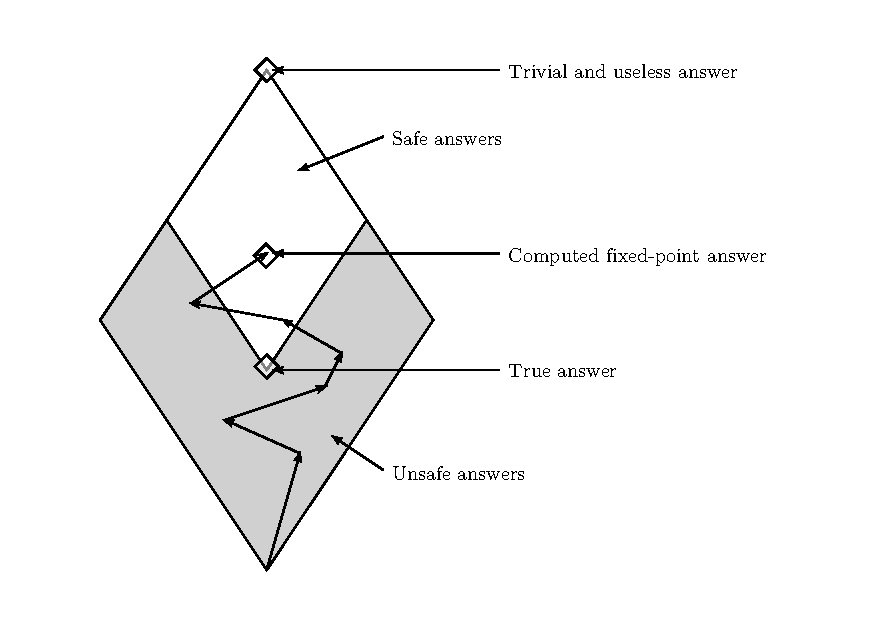
\includegraphics[scale=0.85]{LatticeAnswers.pdf}
\caption{Lattice points as answers \citep{Schwartzbach2009}}
\end{center}
\end{figure}

\paragraph{Example} Given the example of the liveness analysis we can see that the problem domain is a set of all the variables that can occur at each program point. If the set of variables was ${a, b, c}$ then the corresponding lattice would look like that in Figure ~\ref{fig:livenessLattice}.

\begin{figure}
\begin{center}
\graph[scale=0.65]{Lattice}{
"{a,b,c}" -- "{a,b}"
"{a,b,c}" -- "{a,c}"
"{a,b,c}" -- "{b,c}"
"{a,b}" -- "{a}"
"{a,c}" -- "{a}"
"{a,b}" -- "{b}"
"{b,c}" -- "{b}"
"{a,c}" -- "{c}"
"{b,c}" -- "{c}"
"{a}" -- "{}"
"{b}" -- "{}"
"{c}" -- "{}"
}
\caption{Subset lattice for a set of three variables}
\label{fig:livenessLattice}
\end{center}
\end{figure}

\begin{figure}
\begin{center}
\subfloat[$X$]{ \graph[scale=0.65]{LatticeTuples1}{"{}" -- "{a}"} }
\subfloat[$Y$]{ \graph[scale=0.65]{LatticeTuples2}{"{}" -- "{b}"} }
\subfloat[$X \times Y$]{ \graph[scale=0.65]{LatticeTuples3}{"{},{}" -- "{a},{}" -- "{a},{b}"; "{},{}" -- "{},{b}" -- "{a},{b}"} }
\caption{Product of two lattices ($\langle x_1, y_1 \rangle \leq \langle x_2, y_2 \rangle$ iff $x_1 \leq x_2$ and $y_1 \leq y_2$)}
\label{fig:latticeTuples}
\end{center}
\end{figure}

\subsubsection{Computing the fixed-point}

Computing the in- and out-states uses a simple idea that it is only necessary to recompute the out-state if the in-state has changed. The in-state can only change if out-state of any predecessors has changed, or in other words, if the out-state has changed then any successors will have to be recomputed. The generic algorithm for computing the data-flow analysis exploits this fact. Initially all the in-states are initialized to $\emptyset$, except for the one corresponding to the entrypoint, which is initialized to the initial guess. A work list is used to keep a track of all vertices in a control-flow graph for which the in- and out-states have to be recomputed. The work list is initialized with the entrypoint vertex at first. The work list is then processed until it is empty. In each iteration one out-state is computed and all the successors are added to the list for recomputing if the out-state differs from the one computed earlier or if it is the first computed out-state for the particular vertex.

\begin{myalgorithm}
\caption{Computing data-flow analysis using work-list}
\begin{algorithmic}
\FORALL {$v \in Vertices$}
	\STATE $in[v] \gets \emptyset$
	\STATE $out[v] \gets \emptyset$
\ENDFOR
\STATE $in[entry\ vertex] = initial\ guess$
\STATE $worklist = \{entry\ vertex\}$
\WHILE {$worklist \neq \emptyset$}
	\STATE $v \gets deque(worklist)$
	\STATE $out' \gets out[v]$
	\STATE $in[v] \gets \cap out[p]\ for\ all\ p \in predecessor(v)$
	\STATE $out[v] \gets Transfer(in[v], v)$
	\IF {$out[v] \neq out'$}
		\FORALL {$s \in successors(v)$}
			\IF {$s \notin worklist$}
				\STATE $enqueue(worklist, s)$
			\ENDIF
		\ENDFOR
	\ENDIF
\ENDWHILE
\end{algorithmic}
\end{myalgorithm}

\subsubsection{Classification}

\paragraph{May-analysis} identifies possibilities and gathers information that answers whether a specific condition may happen in some code path. It's usually implemented with an initial guess being empty set, a merge function that produces union of the sets (ie. join) and a flow function that adds all possibilities to the set and removes only those possibilities that are guaranteed not to be false.

\paragraph{Must-analysis} provides a guarantee and gathers information that answers whether a specific condition must happen in all code paths. It's usually implemented with an initial guess being empty set, a merge function that produces intersection of the sets (ie. meet) and a flow function that adds only those possibilities that are guaranteed to be true and removes any possibilities that may not happen.

\paragraph{Path-sensitive} analyses use branch conditions and assume that the condition is true on the path if the branch is taken and analogously it is assumed that the condition is false on the path if the branch is not taken. The algorithm for computing the path-sensitive analyses is slightly different from the one presented here and is not covered by this paper.

\section{Interprocedural analysis}

Modern programming languages allow structuring the program code into methods (procedures or functions) that call each other and separate the functionality of the program into isolated chunks. Thus intraprocedural analysis is often not satisfactory for any complex program analysis and serves only as a building block for interprocedural analysis that analyses the program globally.

While the basic algorithm principles are similar for intraprocedural and interprocedural analysis the explored state space is much larger and thus most of the algorithms for interprocedural analyses are about making compromises between accuracy and required computational time.

\subsubsection{Classification}

\paragraph{Flow-sensitive} analyses compute one answer for every program point. It requires intraprocedural data-flow analysis or similar technique. \emph{Flow-insensitive} analysis ignores control-flow and computes one answer for every method. Flow-insensitive analysis is less accurate than the flow-sensitive one, but it can be computed in linear time. There are problems that can be answered adequately with a flow-insensitive analysis, such as whether variable $x$ can be modified by a given method.

\paragraph{Context-sensitive} analyses distinguishes between different call sites of methods. Computing a context-sensitive analysis efficiently is still subject of current research and there are various methods to do it. The simplest approach is to reanalyze callee for each caller, which is often very expensive. Another approach is to compute a generic intraprocedural analysis for each method and then specialize the computed summary for each call site \citep{Gulwani2007}. Yet another technique that is often used are \emph{$k$-context-sensitive algorithms} \citep{Shivers1991,Might2007}, which distinguish call sites up to $k$ levels deep in the call graph and then rerun the callee analysis for each different call site chain. Figure ~\ref{fig:contextSensitivity} shows an example of values gathered by context-sensitive and context-insensitive analyses.

\begin{figure}
\begin{center}
\subfloat[Context-sensitive]{\digraph[scale=0.65]{ContextSensitive}{
   "a = id(4);" -> "id(x) { return x; }" [label="  "];
   "b = id(5);" -> "id(x) { return x; }" [label="  "];
   "id(x) { return x; }" -> "a = id(4);" [label=" 4 ", style=dashed];
   "id(x) { return x; }" -> "b = id(5);" [label=" 5 ", style=dashed];
}}
\subfloat[Context-insensitive]{\digraph[scale=0.65]{ContextInsensitive}{
   "a = id(4);" -> "id(x) { return x; }" [label="  "];
   "b = id(5);" -> "id(x) { return x; }" [label="  "];
   "id(x) { return x; }" -> "a = id(4);" [label=" 4, 5 ", style=dashed];
   "id(x) { return x; }" -> "b = id(5);" [label=" 4, 5 ", style=dashed];
}}
\caption{Difference between context-sensitive and context-insensitive analysis. Context-sensitive analysis provides different answer for a method depending on the context it is called in. Context-insensitive analysis gives a same summary answer for a method regardless of the specific context it is called in. The summary answer is true for all possible calling contexts of the method.}
\label{fig:contextSensitivity}
\end{center}
\end{figure}

\paragraph{Path-sensitive} interprocedural analysis computes one answer for each possible execution path. This is approach taken by model checkers and it is extremely expensive both in terms of memory and computational resources. While many techniques were developed to reduce the searched state space the path-sensitive analysis is still not practical for whole program analysis.

\paragraph{Top-down and bottom-up} Similarly to forward and backward intraprocedural data-flow analysis the graph in interprocedural analysis can be processed in several orders. The \emph{bottom-up} order starts at the leaf methods and summarizes effects of called methods for callers. Conversely the \emph{top-down} order starts at the root methods and summarizes effects of caller for callees.

\subsection{Call graph}

\emph{Static call graph} (also referred to as Procedure Call Graph or PCG) is a directed graph that represents calling relationships between methods in a computer program. For a program with methods $(m_1...m_n)$ the static call graph is defined as $G = (V, S, E, entrypoint)$, where $V = (m_1...m_n)$, $S$ is set of call site labels (ie. labels of program points where a call is performed), $E \subseteq V \times V \times S$ and $entrypoint \in V$ being the program entrypoint.

Construction of a call graph is trivial for languages that don't feature dynamic dispatch (ie. virtual methods in object oriented languages, function pointers or other forms of indirect calls). For languages with dynamic dispatch, such as Java or C\#, computing a static call graph precisely requires alias analysis results. Conversely, computing precise aliasing requires a call graph. To solve this problem both alias analysis and call graph construction have to be performed simultaneously.

An over-approximated call graph can be computed trivially even for languages with dynamic dispatch by employing various techniques, such as resolving virtual method calls using the class hierarchy graph based on declared variable type. We will refer to this over-approximation as \emph{CHA call graph}. A simple extension of this approach is the \emph{Rapid-Type Analysis} \citep{Bacon1997}, where the CHA call graph is reduced by using the fact that an instance method cannot be called unless the type is instantiated in the program.

\subsection{Data-flow}

There are several methods for computing data-flow analyses on interprocedural level. The most fundamental ones will be explored in this section, but unlike intraprocedural analysis there is no single canonical algorithm.

\subsubsection{Control-flow super graph}

\emph{Control-flow super graph} is constructed by combining control-flow graphs of all the methods into one huge graph by adding edges between call site and method entrypoint and exitpoint(s). The advantage of this representation is that intraprocedural data-flow analysis can be used unmodified on the super graph. It's not very practical though, because the performance of the work-list data-flow computation dependents directly on the number of cycles in the graph and each call site adds one cycle to the super graph. Also the super graph smears information from different contexts and thus such data-flow analysis would be context-insensitive.

\begin{figure}
\begin{center}
\digraph[scale=0.65]{ControlFlowSuperGraph}{
  subgraph cluster_foo {
    "x = 3" -> "bar(x)" -> "bar(1)"
    label="foo"
  }
  subgraph cluster_bar {
    "y = x + 1" -> "return"
    label="bar"
  }
  "bar(x)" -> "y = x + 1"
  "return" -> "bar(x)"
  "bar(1)" -> "y = x + 1"
  "return" -> "bar(1)"
}
\caption{Example of a control-flow super graph}
\label{fig:controlFlowSupergraph}
\end{center}
\end{figure}

\subsubsection{Invocation graph}

A brute-force approach for computing interprocedural data-flow analysis is to use an \emph{invocation graph} (Figure ~\ref{fig:invocationGraph}), where a distinct path exists for each possible call chain. It is inherently context-sensitive and also very precise, but due to the nature of the invocation graph it is also exponentially expensive in relation to program size and it is problematic to compute the analysis for recursive call chains. 

\begin{figure}
\begin{center}
\subfloat{
\parbox[b]{50mm}{
main() \{ foo(4); foo(5); \} \\
foo(x) \{ bar(x); \} \\
bar(x) \{ ... \} \\ \\ \\
}
\subfloat{
\digraph[scale=0.65]{InvocationGraph}{
foo2 [label="foo"]
bar2 [label="bar"]
main -> foo -> bar
main -> foo2 -> bar2
}
}
}
\caption{Example of an invocation graph}
\label{fig:invocationGraph}
\end{center}
\end{figure}

%\subsubsection{Partial transfer function}

%A \emph{partial transfer function} (PTF) describes the behavior of a method assuming that certain properties hold in the context where it is called. It can be reused in many calling contexts as long as the properties of the inputs to the method are the same. It was demonstrated for alias analysis that by precomputing a single partial transfer function for each method a fully context-sensitive analysis can be implemented efficiently \citep{Wilson1995}.

%  [Wilson et al'95]
% Use memoization.
% funcOutput = PTF(funcInput).
% PTF computed once for an "input pattern".
% Lazily compute PTFs for each procedure.

\subsubsection{Static call graph}

Interprocedural analysis can be computed directly on the static call graph by decoupling the intraprocedural part from the interprocedural part. The work-list algorithm that is used for computing the intraprocedural analysis is reused for traversing the static call graph. At each vertex an intraprocedural analysis is performed to compute a method summary, which is then merged back into the caller's symbolic state (Figure ~\ref{fig:StaticCallGraphUpdates}).

\begin{figure}
\begin{center}
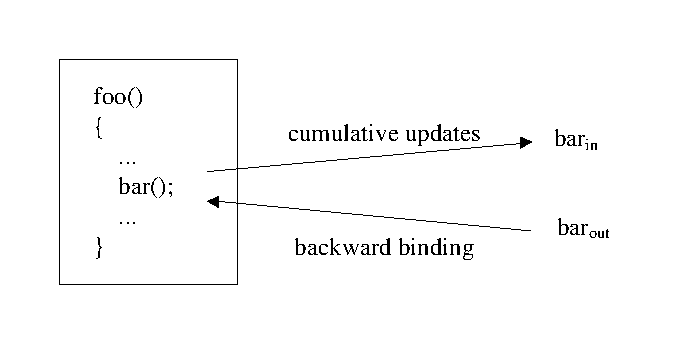
\includegraphics[scale=0.8]{StaticCallGraphUpdates.pdf}
\end{center}
\caption{Updates in an interprocedural analysis on static call graph. The calling context summary, represented by $bar_{in}$ is union of all possible in-states at all call sites of $bar$. The method summary, represented by $bar_{out}$, is computed by intraprocedural analysis of $bar$ with the initial guess $bar_{in}$. It is merged back into the out-state at each call site of $bar$.}
\label{fig:StaticCallGraphUpdates}
\end{figure}

% Procedure call graph [Choi et al'93]
% Each procedure - a PCG vertex.
% Each call site - an edge in PCG.

% Context insensitive.

The basic algorithm for computing the data-flow analysis on a static call graph is outlined in Algorithm ~\ref{fig:DataFlowPCG}. We show an iterative algorithm for simplicity, in practice the work-list algorithm is used. The flow function in the intraprocedural analysis has to be modified to account for calls by lazily reevaluating them using the values computed on the static call graph. The initial guess for the intraprocedural analysis is substituted with union of all in-states leading to the called method. 

\begin{myalgorithm}
\caption{Computing data-flow analysis on PCG}
\label{fig:DataFlowPCG}
\begin{algorithmic}
\REPEAT
	\FORALL {vertices $p \in PCG$}
		\STATE \COMMENT{Perform intraprocedural analysis, in this case a flow-insensitive one}
		\REPEAT
			\FORALL {vertices $n \in p.CFG$}
				\IF {statement $n$ is a call to $m$}
					\STATE Compute $n_{out}$ using $m_{out}$ and $n_{in}$
				\ELSE
					\STATE $n_{out} \gets F(n_{in})$
				\ENDIF
			\ENDFOR
		\UNTIL {for each vertex $n \in p.CFG$, $n_{in}$ and $n_{out}$ converge}

		\STATE \COMMENT{Construct the method summary}
		\STATE $p_{out} \gets$ merge of all $out$ flow values from exitpoints of $p$
		\STATE \COMMENT{Update the in-state for all called methods}
		\FORALL {methods $m$ called by $p$}
			\STATE $m_{in} \gets m_{in} \sqcup n_{in}$
		\ENDFOR
	\ENDFOR
\UNTIL {for each vertex $p \in PCG$, $p_{in}$ and $p_{out}$ converge}
\end{algorithmic}
\end{myalgorithm}

\begin{figure}
\begin{center}
\subfloat{
\parbox[b]{50mm}{
main() \{ foo(4); foo(5); \} \\
foo(x) \{ bar(x); \} \\
bar(x) \{ ... \} \\ \\ \\
}
\subfloat{
\digraph[scale=0.65]{ProcedureCallGraph}{
main -> foo -> bar
main -> foo
}
}
}
\caption{Example of a procedure call graph}
\label{fig:procedureCallGraph}
\end{center}
\end{figure}

\subsubsection{Static call graph with context-sensitivity}

The algorithm we presented in previous section can be modified to provide context-sensitivity \citep{Chatterjee1999,Cheng2000}. Instead of computing a method summary based on a specified initial guess we construct a \emph{context independent summary function} (CISF). The intraprocedural analysis computes a symbolic summary with unknown initial guess that can be transferred by the CISF for a specific context it is called in.

\subsection{Alias analysis}

Languages that support pointers or references introduce a complication for static analysis. Two (or more) variables may refer to the same memory location at the same time. A pessimistic assumption that two variables may always point to the same location is sound, but often hinders the particular analysis to the point that it is ineffective. A slightly better assumption that can be made for many languages is that two variables may alias if they are declared to be the same type or if they can be casted to a common parent type or interface.

Additional complication are objects created on the heap. There is a potentially unbounded number of them and so in order to be able to reason about them we have to represent them using a bounded approximation. One such approximation is to use the allocation site (ie. program point of the allocation, possibly together with call site for context-sensitive algorithms).

\emph{Alias analysis} is a static analysis that computes information about possible aliases for variables, which in effect helps other analyses make less conservative decisions.

The best known flow-based alias analyses are described by \citet{Andersen1994} and \citet{Steensgaard1996}, which are briefly described below.

\begin{figure}
\begin{center}
\unitlength 1mm % = 2.845pt
\linethickness{0.4pt}
\begin{picture}(80,60)(0,0)
\put(5,5){\vector(0,1){55}}
\put(5,5){\vector(1,0){75}}
\put(19,16){\oval(28,6)[]}
\put(19,16){\makebox(0,0)[cc]{Steensgard '96}}
\put(23,10){\oval(26,6)[]}
\put(23,10){\makebox(0,0)[cc]{Andersen '94}}
\put(40,30){\oval(20,6)[]}
\put(40,30){\makebox(0,0)[cc]{Burke '95}}
\put(65,30){\oval(20,6)[]}
\put(65,30){\makebox(0,0)[cc]{Choi '93}}
\put(60,55){\oval(22,6)[]}
\put(60,55){\makebox(0,0)[cc]{Emami '94}}
\put(69,49){\oval(22,6)[]}
\put(69,49){\makebox(0,0)[cc]{Wilson '95}}
\put(40,2){\makebox(0,0)[cc]{Flow-sensitivity}}
\put(2,30){\makebox(0,0)[cc]{\begin{sideways}Context-sensitivity\end{sideways}}}
\end{picture}
\caption{Overview of various alias analyses}
\label{fig:aliasOverview}
\end{center}
\end{figure}

\subsubsection{Representation}

There are several commonly used representations for the aliasing information. The following code written in C notation will be used as an example: $q=\&p; p=\&i; r=\&i;$.

\begin{itemize*}

\item \emph{Complete alias pairs} \citep{Landi1992} store all alias pairs explicitly. Example: $\langle*q, p\rangle, \langle*p, i\rangle, \langle*r, i\rangle, \langle**q, p\rangle, \langle**q, i\rangle, \langle*p, *r\rangle, \langle**q, *r\rangle$

\item \emph{Compact alias pairs} \citep{Choi1993} store only basic aliasing pairs. The complete aliasing pairs are derived using dereferencing, transitivity and commutativity. Example: $\langle*q, p\rangle, \langle*p, i\rangle, \langle*r, i\rangle$

\item \emph{Points-to relations} \citep{Emami1993} indicate that one variable points to another. Example: $(q, p), (p, i), (r, i)$

\end{itemize*}

\subsubsection{Steensgaard's analysis}

Steensgaard alias analysis has the following characteristics:
\begin{itemize*}
\item The algorithm is context-insensitive and flow-insensitive.
\item One points-to set is computed per pointer variable (eg. method argument, local variable, static field or instance field) over the entire program.
\item Pointer assignment is represented by unification constraints ($p = q$ implies $points\mhyphen{}to(p) = points\mhyphen{}to(q)$).
\item Fast union-find data structure is used for implementation. 
\item Solution is computed in almost linear time in terms of program size.
\item Imprecision stems from merging points-to sets.
\end{itemize*}
The general outline of the algorithm is the following:
\begin{itemize*}
\item Find all pointer assignment statements in the program.
\item Form points-to set $\{p\}$ for each pointer variable $p$.
\item Examine each assignment statement (eg. explicit assignment or implicit assignment during parameter passing), in an arbitrary order, and merge points-to sets for the involved variables.
\end{itemize*}

\subsubsection{Andersen's analysis}

Andersen's analysis offers more precision than Steensgard's analysis. It shares the context- and flow-insensitiveness characteristic. Pointer assignment is represented by inclusion constraints ($p = q$ implies $points\mhyphen{}to(p) \subseteq points\mhyphen{}to(q)$). The computed points-to graph is larger than Steensgaard's, but more precise. The analysis has in the worst case cubic complexity in terms of program size.

\subsubsection{FA analysis}

FA alias analysis is very similar to the Steensgaard's analysis. It is also computed using the union-find data structure, but compared to the Steensgaard's analysis it distinguishes between individual structure fields. The importance of the FA analysis lies in the fact, shown by \citet{Milanova2002}, that even though the analysis is relatively imprecise it yields sufficiently precise results for constructing call graphs of programs containing function pointers.

\myepigraph{In fact what I would like to see is thousands of computer scientists let loose to do whatever they want. That's what really advances the field.}%
         {Donald Knuth}
\chapter{Related works}
         
\section{Run-time deadlock detection}

The classic approach to deadlock detection in object-oriented programs is run-time detection with the \emph{GoodLock} algorithm \citep{Havelund2000}. The algorithm works by building a lock order graph by intercepting the locking calls of a running program. The resulting graph is examined for a presence of cycles. The original algorithm detects only deadlocks caused by two resources; a variant called \emph{generalized GoodLock} \citep{Agarwal2005,Agarwal2006} extends the algorithm to handle an arbitrary number of resources. Most run-time algorithms are only variations of the GoodLock algorithm that improve upon it by reducing false positives and providing additional information to track a source of the deadlocks.

\section{Data-flow analyses}

Using static program analysis to find deadlocks in programs isn't a novel approach either. Several techniques have been developed \citep{Artho2001,Praun2004,Jlint} and each of them has its own benefits and drawbacks. In the context of object-oriented languages, most of the work was focused on Java.

To the best of our knowledge, the Jlint static checker \citep{Jlint} is the first tool to use the lock order graph. The original implementation of the tool considers only synchronized methods and it doesn't model synchronized blocks (equivalent of lock blocks in C\#). Artho and Biere \citep{Artho2001} extended the tool to support synchronized blocks. The Jlint analysis is very simplistic and detects only a small subset of potentials deadlocks. The main drawbacks include: 1) fields and local variables are considered to be unaliased, 2) nested synchronized blocks are not tracked across class boundaries, and 3) inheritance is not fully considered.

A part of the original Jlint tool was ported to .NET Framework 1.0 as CSLint \citep{CSLint}. It was even more limited than the original Java tool. Several ports to .NET Framework 2.0 were later introduced, which added a partial support for generics, but the limitations of the original Jlint tool remained.

Christopher von Praun has written a PhD thesis \citep{Praun2004} dedicated to finding multi-threading problems, such as race conditions, atomicity violations and deadlocks, in Java programs. His work has provided significant contribution to further research of static analysis of parallel programs. One of the key ideas suggested by the thesis was that alias analysis is a key component of the static deadlock detection techniques.

A sophisticated interprocedural data-flow analysis is described by \citet{Williams2005} that builds a lock order graph. The analysis is targeted at verifying program libraries as opposed to whole programs. Contrary to Jlint the analysis correctly takes inheritance into account and the interprocedural approach provides better value tracking and also properly treats the reentrancy of locks.

Naik has co-written a significant number of research papers with regard to static analysis of concurrent programs \citep{Naik2006,Naik2008,Naik2009}. The effort has resulted in development of the JChord tool \citep{jchord}. The tool uses an innovative combination of static analyses ($k$-CFA call graph and alias analysis, thread escape analysis, may happen in parallel analysis) to search for data races and deadlocks. It attacks the deadlock detection problem by scanning each tuple $(t_a,l_a^1,l_a^2,t_b,l_b^1,l_b^2)$, where $t_a$ and $t_b$ are threads and $l_a^1$, $l_a^2$, $l_b^1$ and $l_b^2$ are locks, for satisfying six deadlock conditions:
\begin{itemize*}
\item \emph{reachability} \newline Is it possible to find a code path, where lock $l_a^1$ is taken and then lock $l_a^2$ is acquired in thread $t_a$ (and equivalently for $l_b^1$, $l_b^2$ and $t_b$)?
\item \emph{aliasing} \newline Can lock $l_a^1$ be the same lock as $l_b^2$ (and equivalently for $l_b^1$ and $l_a^2$)?
\item \emph{escaping} \newline Can lock $l_a^1$ be accessible from more than one thread (and similarly for $l_a^2$, $l_b^1$ and $l_b^2$)?
\item \emph{parallel} \newline Can different threads $t_a$ and $t_b$ simultaneously reach $l_a^2$ and $l_b^2$?
\item \emph{non-reentrancy}
\item \emph{no guard lock}
\end{itemize*}
The first four conditions are verified soundly, while the last two are approximated. The $k$-CFA analysis is run iteratively with increasing $k$ context-sensitivity for as long as the number of reports decreases. This significantly reduces the number of false positives while the analysis remains computationally feasible. A shortcoming of the analysis is that it cannot detect deadlocks caused by three or more locks waiting in a circular chain.

\section{Model checking}

Several groups have taken a model-checking approach to finding deadlocks in Java programs. The best known tool is Java Pathfinder \citep{Havelund1999,Brat2000} that translates Java into Promela language, which is then verified using the SPIN model checker. The tool is very precise at the expense of analysis time.

A model checking for \emph{Mono}, an open-source .NET Framework implementation, was implemented in the MoonWalker tool \citep{AanDeBrugh2009}. The tool analyzes .NET byte code and interprets it along all possible code paths. This makes it unsuitable for use on large programs. There were further problems with the implementation itself, most notably: 1) the tool is tied closely to the Mono run-time due to dependency on the specific Base Class Library implementation and its internals, and 2) bugs in the type handling code prevent it from working even on the simplest programs\footnote{For example, the type handling code doesn't keep track of type of delegates, thus it incorrectly emulates a code such as \texttt{if (delegateVariable is ThreadStart) \{ ... \}}.}.

The common problem with the model checking approach is that it is not scalable to large programs. Various techniques have been developed to reduce the search space, such as over-abstracting the model or combining it with data-flow analysis to identify places where additional precision is needed \citep{Brown2007}.

\section{Petri nets}

Petri Nets have a large body of research, both theoretical and practical, sup-porting their use for concurrent system analysis. Bateman and Pouarz have presented a paper \citep{Bateman2002} that examined how to transform Java concurrency to Petri Net representation. The Petri Nets offer very flexible representation that allows modeling complex synchronization primitives such as Semaphore, ReaderWriterLock or even unbalanced locks across multiple methods. However, they do not inherently allow modeling of reentrant locks. While many deadlock preserving reductions exist that reduce the search space, finding a deadlock in a Petri Net is still a problem with exponential complexity.    

\section{Companion tools for testing}

A new class of tools has recently appeared that uses the results of imprecise static or dynamic program analyses. The imprecise analysis is run first on the program to identify potential concurrency bugs. In a second phase the reports from the imprecise analysis are used to explicitly control the underlying scheduler of the concurrent program to accurately and quickly reproduce real concurrency bugs, if present, with high precision. Prominent examples of these tools are CalFuzzer \citep{Joshi2009} for Java, CHESS \citep{Musuvathi2007} for Win32 and .NET applications, and TypeMock Racer \citep{TypeMockRacer} for .NET.
\myepigraph{Essentially, all models are wrong, but some are useful.}%
         {George Box}
\chapter{Design}

\section{Goals}

The following goals and limitations are targeted by the analysis:
\begin{itemize*}
\item Only safe and verifiable code should be analyzed. Unsafe code is largely used for interoperability with native libraries and thus its analysis wouldn't significantly contribute to the accuracy, if at all. The tool should be able to cope with unsafe code and skip over it if encountered.
\item Dynamically generated code will not be analyzed.
\item The whole program will be analyzed. Other works have investigated the use of program verification of software libraries. It would be an advantage if the chosen algorithm could later be extended to handle this scenario as well, but it is not a target of the prototype.
\item The analysis should scale to applications as large as 200,000 lines of code.
\item Locks managed by \texttt{Monitor.Enter}, \texttt{Monitor.TryEnter} and \texttt{Monitor.Exit} methods will be considered by the analysis. Other locking primitives are considered out of scope for the prototype.
\item It is assumed that locks are balanced and that for each \texttt{Monitor.Enter} and \texttt{Monitor.TryEnter} call there is a corresponding \texttt{Monitor.Exit} call and that the exit calls are made in reverse order of the enter calls. 
\end{itemize*}

\section{Algorithm overview}

The chosen algorithm is based on paper by \citet{Williams2005}. A high-level overview of the algorithm is given below and the specifics of applying the analysis to .NET code are discussed.

Only two of the conditions necessary for deadlock to occur, namely \emph{lock order inversion} and \emph{no guard lock}, are verified. 

First a lock order graph of the program is constructed using an interprocedural data-flow analysis. The analysis is flow-sensitive and context-sensitive. At each program point a symbolic state is computed that models the execution state along with an associated lock order graph and root set. The symbolic state at the end of a method is used as a method summary. The work list algorithm is used to compute a fixed point over all methods in the program. Thread entrypoints are identified in the call graph and method summaries of the entrypoints are merged into a single lock order graph that is output of the analysis.

Context-sensitivity is provided by computing the intraprocedural analysis with a symbolic representation of method arguments, which are then substituted for the actual arguments at each call site.

Each vertex of the lock order graph represents a set of objects that may be aliased. An edge represents nested locking of objects along some code path.

The original analysis uses types as an approximation for the may-alias sets and we follow suit.

Value flow through fields is not considered and can be computed using a separate analysis for a better precision.

\section{Algorithm details}

\subsection{Code representation}

The analysis is executed directly on top of the intermediate language byte code instead of first translating the code to higher-level abstraction such as three-address code or abstract syntax tree\footnote{Description of different code representations can be found in \citet{Aho1986} and \citet{Muchnick1998}.}. While this makes the analysis faster it also makes it more complicated and introduces the following challenges:
\begin{itemize*}
\item In addition to modeling local variables the evaluation stack has to be modeled as well.
\item The analysis as described by Williams doesn't have to account for separate \texttt{Monitor.Enter} and \texttt{Monitor.Exit} calls. Instead, it deals with the high-level \texttt{synchronized (object)} code blocks.
\item The new \texttt{lock (object)} construct as implemented in C\# 4 causes the data-flow analysis to join on code paths where the stacks of currently acquired locks have different depth (eg. the code path where \texttt{if (acquired)} is taken and the one where it is not). Since our analysis is path-insensitive we cannot infer that one of the code paths is never taken. We account for it by joining the stacks only up to all elements that are common to both stacks. 
\end{itemize*}

The data-flow rules presented later in this section reference the instructions by their canonical name. Macro instructions, such as \texttt{Ldarg\_0}, are not included for bravity.

\subsection{Symbolic state}

The symbolic state (Figure ~\ref{fig:symbolicState}) is 7-tuple consisting of:
\begin{itemize*}
\item Current lock-order graph
\item Root set of the lock-order graph
\item Set of objects that have had \texttt{Monitor.Wait} called on them without an enclosing lock held in the current method
\item Locks that are currently held in the order in which they were obtained, including re-entered locks
\item Map of local variables to their symbolic object values
\item Current evaluation stack in the method
\item Map of method argument variables to their symbolic object values
\end{itemize*}

Since the state is composed of finite sets and finite graphs, it is possible to represent it as a lattice composed from individual power-set lattices. The join operation is defined accordingly in Listing ~\ref{fig:joinFunction} as the join of individual sets in the tuple. The initial symbolic state for each method is defined in ~\ref{fig:initialState}.

\begin{figure}
\begin{tabulary}{\textwidth}{ R C L }
$T$ & $\in$ & Type \\
$programPoint$ & $\in$ & ProgramPoint$_\bot$ \\
$o$ = $\langle$ $programPoint$, $T$ $\rangle$ & $\in$ & SymbolicObject = ProgramPoint $\times$ Type \\
$lockGraph$ & $\in$ & Graph = directed-graph-of SymbolicObjects \\
$roots$ & $\in$ & Roots = set-of SymbolicObjects \\
$wait$ & $\in$ & Wait = set-of SymbolicObjects \\
$locals$ & $\in$ & Locals = LocalVariable $\rightarrow$ SymbolicObject \\
$stack$ & $\in$ & Stack = stack-of (SymbolicObject $|$ null) \\
$arguments$ & $\in$ & Arguments = Argument $\rightarrow$ SymbolicObject \\
$s$ = $\langle$ $lockGraph$, $roots$, $wait$, $locks$, $locals$, $stack$, $arguments$ $\rangle$ & $\in$ & State = Graph $\times$ Roots $\times$ Wait $\times$ list-of SymbolicObjects $\times$ Locals $\times$ Stack $\times$ Arguments \\
\end{tabulary}
\caption{Type domains and symbolic state definition}
\label{fig:symbolicState} 
\end{figure}

\begin{lstlisting}[language=CSharp,mathescape,caption=Join function for state,label=fig:joinFunction,float]
$s_1 \sqcup s_2$ returns State $s'$
  $s'$.g $\leftarrow$ $s_1$.g $\cup$ $s_2$.g
  $s'$.roots $\leftarrow$ $s_1$.roots $\cup$ $s_2$.roots
  $s'$.wait $\leftarrow$ $s_1$.wait $\cup$ $s_2$.wait
  $s'$.locks $\leftarrow$ longest common sequence of $s_1$.locks and $s_2$.locks
  $s'$.locals $\leftarrow$ $s_1$.locals $\sqcup$ $s_2$.locals
  $s'$.stack $\leftarrow$ $s_1$.stack $\sqcup$ $s_2$.stack
  $s'$.arguments $\leftarrow$ $s_1$.arguments $\sqcup$ $s_2$.arguments
  
$locals_1 \sqcup locals_2$ returns Locals $locals'$
  $\forall$ $v \in ${$v' | v' \in locals_1 \vee v' \in locals_2$}
    $locals' \leftarrow locals' \cup (locals_1[v] \sqcup locals_2[v])$

$arguments_1 \sqcup arguments_2$ returns Arguments $arguments'$
  $\forall$ $v \in ${$v' | v' \in arguments_1 \vee v' \in arguments_2$}
    $arguments' \leftarrow arguments' \cup (arguments_1[v] \sqcup arguments_2[v])$

$stack_1 \sqcup stack_2$ returns Stack $stack'$
  /* all stacks have equivalent depth */
  while (!stack_empty($stack_1$))
    $v_1$ $\leftarrow$ $stack_1$.pop()
    $v_2$ $\leftarrow$ $stack_2$.pop()
    if ($v_1$ == null) $stack'$.push($v_2$)
    else $stack'$.push($v_1 \sqcup v_2$)
  $stack'$.reverse()

$o_1 \sqcup o_2$ returns SymbolicObject $o'$
  if ($o_1$ == $o_2$) $o' \leftarrow o_1$
  else $o' \leftarrow \langle$ program_point(join_point($v$)), $T_1 \sqcup$ $T_2$ $\rangle$
 
$T_1 \sqcup T_2$ returns lowest common superclass of $T_1$ and $T_2$

$lockGraph_1 \sqcup lockGraph_2$ returns Graph $lockGraph'$
  /* equivalent SymbolicObject values are collapsed */
  vertices($lockGraph'$) $\leftarrow$ vertices($lockGraph_1$) $\cup$ vertices($lockGraph_2$)
  /* equivalent SymbolicObject pairs are collapsed */
  edges($lockGraph'$) $\leftarrow$ edges($lockGraph_1$) $\cup$ edges($lockGraph_2$)

\end{lstlisting}

\begin{lstlisting}[language=CSharp,mathescape,caption=Initial symbolic state for method,label=fig:initialState,float]
initial_state($F$) returns State $s_0$
    $s_0 \leftarrow$ empty State
		$\forall$ $p \in F$.$arguments$
      $o$ $\leftarrow$ $\langle$ entrypoint($F$), typeof($p$) $\rangle$
      $s$.$arguments$[$p$] $\leftarrow$ $o$
\end{lstlisting}

\subsubsection{Symbolic object model}

Each symbolic heap object represents the set of objects created at a given program point and their type.

\subsubsection{Lock stack model}

The analysis has to keep track of what locks are currently acquired in the method. This is done using the $locks$ stack. Each entry in the stack refers to a symbolic object that \texttt{Monitor.Enter} or \texttt{Monitor.TryEnter} method was called on. Re-entered locks are not recorded to the lock graph, but they are tracked in the $locks$ stack to allow for proper reference counting.

We define \texttt{top\_lock($locks$)} as the last entered lock that wasn't already on the $locks$ stack.

\subsubsection{Stack model}

The .NET virtual machine can store different data types on the evaluation stack, such as 32-/64-bit/native integers, floating point numbers, managed pointers, transient pointers and object references.

Integers and floating point numbers are largely irrelevant to our analysis. It is impossible to lock on value types, so an explicit boxing is necessary before these values are used. We do not model effect of such a boxing, but it is possible to enhance the analysis to account for it by handling the \texttt{box} instruction. We haven't observed any code that would use such construct although it is theoretically possible.

Managed pointers are primarily used for passing parameters by indirect reference (the \texttt{ref} or \texttt{out} keywords in C\#). We do not model these stack values for simplicity. However, it was observed that at least one place in the Base Class Library calls \texttt{Monitor.Enter} on a method parameter that is passed by reference, and thus it is desirable to extend the analysis to support these stack values in the future.

Transient pointers are used for referencing unmanaged memory and as such are of no interest to us.

Finally, object references are modeled as symbolic object references on our stack.

The $null$ meta-symbol is used for unknown stack entry, which could be either one of the unsupported data types listed above or object reference resulting from an unhandled instruction.

\subsection{Flow function}

The data-flow rules that compose the flow function are the following:
\begin{itemize*}
\item Basic value flow through stack, local variables and argument variables is described in Listing ~\ref{fig:rulesVariables}.
\item Loading of values from fields, static fields and array elements is described in Listing ~\ref{fig:rulesLoad}.
\item Method calls, creation of new objects and creation of new arrays are described in Listing ~\ref{fig:rulesCallAndNew}.
\item For all unhandled instructions the evaluation stack is modified accordingly. First the correct number of elements is popped from the stack and then the correct number of $null$ meta-elements is pushed on the stack.
\end{itemize*}

The \texttt{Monitor} methods are intercepted when handling the \texttt{Call} instruction and handled by the helper methods in Listing ~\ref{fig:rulesHelpers}.

Method calls are resolved using a pre-built call graph (eg. CHA call graph) and their summary state is merged into the caller call graph when handling the call instructions. The formal method parameters are mapped to the actual parameters, which increases precision. Return value from the summary state is currently not used, but it could serve to improve the precision as well. 

\begin{lstlisting}[language=CSharp,mathescape,caption=Data-flow rules for local variable handling,label=fig:rulesVariables,float]
Ldarg $Argument$
    /* Load method argument onto stack. */
    $o$ $\leftarrow$ $s$.$arguments$[$Argument$]
    $s$.$stack$.push($o$);
    
Starg $Argument$
    /* Pops the top value from the stack and stores it in argument slot for argument Argument. */
    $o$ $\leftarrow$ $s$.$stack$.pop()
    $s$.$arguments$[$Argument$] $\leftarrow$ $o$

Ldloc $LocalVariable$
    /* Loads the local variable onto stack. */ 
    $o$ $\leftarrow$ $s$.$locals$[$LocalVariable$]
    $s$.$stack$.push($o$)

Stloc $LocalVariable$
    /* Pops a value from the stack and stores it in local variable. */
    $o$ $\leftarrow$ $s$.$stack$.pop()
    $s$.$locals$[$LocalVariable$] $\leftarrow$ $o$

Dup
    /* Duplicates the value on the top of the stack. */
    $o$ $\leftarrow$ $s$.$stack$.pop()
    $s$.$stack$.push($o$)
    $s$.$stack$.push($o$)    

Isinst $T$
    /* Tests if an object reference is an instance of T, returning either a null reference or an instance of that class or interface. */
Castclass $T$
    /* Casts an object to a new object of type T. */
    $o$ $\leftarrow$ $s$.$stack$.pop()
    if ($o$ == null)
      $s$.$stack$.push($o$)
    else
      $s$.$stack$.push($\langle$ $o$.$programPoint$, $T$ $\rangle$)
\end{lstlisting} 

\begin{lstlisting}[language=CSharp,mathescape,caption=Data-flow rules for other variable loading,label=fig:rulesLoad,float]
Ldfld $F$
    /* Pushes the value of a field F in a specified object o1 onto the stack. */
  	$o_1$ $\leftarrow$ $s$.$stack$.pop()
		$o$ $\leftarrow$ $\langle$ program_point($stmt$), declared_type($T$) $\rangle$
    $s$.$stack$.push($o$)

Ldsfld $F$
    /* Push the value of field F on the stack. */
		$o$ $\leftarrow$ $\langle$ program_point($stmt$), declared_type($T$) $\rangle$
    $s$.$stack$.push($o$)

Ldelem_Ref $T$
    /* Loads the element with an object reference at index onto the top of the stack as type T. */
    $index$ $\leftarrow$ $s$.$stack$.pop()
  	$o_1$ $\leftarrow$ $s$.$stack$.pop()
		$o$ $\leftarrow$ $\langle$ program_point($stmt$), element_type($o_1$) $\rangle$
    $s$.$stack$.push($o$)
\end{lstlisting}

\begin{lstlisting}[language=CSharp,mathescape,caption=Data-flow rules for calls and object creation,label=fig:rulesCallAndNew,float]
Newobj $F$
    /* Allocates an uninitialized object or value type and calls the constructor method. */
Calli $F$
    /* Calls the method pointed to with arguments described by the calling convention. */
Call $F$
    /* Call the method F */
Callvirt $F$
    /* Calls a specific method associated with o. */

    /* intercept Monitor calls */
    if (opcode == Call)
      if ($F$ == Monitor.Enter || $F$ == Monitor.TryEnter)
        enter_lock($s$, first_parameter($s$, $F$))
      else if ($F$ == Monitor.Exit)
        exit_lock($s$, first_parameter($s$, $F$))
      else if ($F$ == Monitor.Wait)
        wait_on_lock($s$, first_parameter($s$, $F$))

    /* pop indirect address for calli */
    if (opcode == Calli)
      $s$.$stack$.pop();
        
		/* pop method arguments */
		$\forall$ $p \in F$.$arguments$
			$s$.$stack$.pop();
		if (!is_static($F$))
			$o$ $\leftarrow$ $s$.$stack$.pop();
		else
			$o$ $\leftarrow$ null;

    $\forall$ $F_v \in$ versions of $F$ in subclasses of $o$
      $s_m$ $\leftarrow$ method_summary($F_v$)
      $s_m$ $\leftarrow$ rename_from_callee_to_caller_context($s_m$, $state$, $F_v$) 
      /* connect the two graphs, including roots */
      if (empty($s$.$locks$))
        $s$.$roots$ $\leftarrow$ $s$.$roots$ $\cup$ $s_m$.$roots$
        $s$.$wait$ $\leftarrow$ $s$.$wait$ $\cup$ $s_m$.$wait$
      else
        $\forall$ $root \in s_m$.$roots$
          $s$.$lockGraph$ $\leftarrow$ $s$.$lockGraph$ $\cup$ edge(top_lock($s$.$locks$) $\rightarrow$ $root$)
        $\forall$ $w \in s_m$.$wait$
          $s$.$lockGraph$ $\leftarrow$ $s$.$lockGraph$ $\cup$ $w$ $\cup$ edge(top_lock($s$.$locks$) $\rightarrow$ $w$)
				
		/* push return value */
		if (return_type($F$) != void)
    		$o$ $\leftarrow$ $\langle$ program_point($stmt$), return_type($F$) $\rangle$
				$s$.$stack$.push($o$);

Newarr $T$
    /* Creates a new array with elements of type T. */
    $s$.$stack$.pop()
		$o$ $\leftarrow$ $\langle$ program_point($stmt$), $T$ $\rangle$
    $s$.$stack$.push($o$)
\end{lstlisting}

\begin{lstlisting}[language=CSharp,mathescape,caption=Helper methods,label=fig:rulesHelpers,float]
enter_lock($s$, $o$)
    if ($o \notin s$.$locks$)
      if (empty($s$.$locks$))
        $s$.$lockGraph$ $\leftarrow$ $s$.$lockGraph$ $\cup$ $o$
        $s$.$roots$ $\leftarrow$ $s$.$roots$ $\cup$ $o$
      else
        $s$.$lockGraph$ $\leftarrow$ $s$.$lockGraph$ $\cup$ $o$ $\cup$ edge(top_lock($s$.$locks$) $\rightarrow$ $o$)
    $s$.$locks$.push($o$)

exit_lock($s$, $o$)
    /* locks are balanced */
    $s$.$locks$.pop()

wait_on_lock($s$, $o$)
    if (empty($s$.$locks$))
      $s$.$wait$ $\leftarrow$ $s$.$wait$ $\cup$ $o$
    else
      /* wait releases and then reacquires, which can introduce new lock ordering */
      $s$.$lockGraph$ $\leftarrow$ $s$.$lockGraph$ $\cup$ $o$ $\cup$ edge(top_lock($s$.$locks$) $\rightarrow$ $o$)
      
rename_from_callee_to_caller_context($s_{caller}$, $s_{callee}$, $F_v$) returns State $s'$
    $s' \leftarrow s_{caller}$
    $stack \leftarrow s_{caller}$.$stack$
    
    /* create a map for formal arguments to their actual values */ 
    $\forall a \in$ reverse($F_v$.$arguments$)
      $map_{\langle entrypoint(F_v), typeof(a) \rangle} \leftarrow stack$.pop()
      
    $\forall o \in s_{callee}$.$lockGraph$
      if ($\exists map_o$) $o' \leftarrow map_o$
      else $o' \leftarrow \langle pp_\bot, o$.T$ \rangle$
      if ($o' \in s_{caller}$.$locks$) $s'$.$lockGraph$, $s'$.$roots$ $\leftarrow$ splice_out_vertex($s'$.$lockGraph$, $s'$.$roots$, $o$)
      else $s'$.$lockGraph$, $s'$.$roots$ $\leftarrow$ replace_vertex($s'$.$lockGraph$, $s'$.$roots$, $o$, $o'$)
    $s'$.$wait \leftarrow \emptyset$        
    $\forall o \in s_{callee}$.$wait$
      if ($\exists map_o$) $s'$.$wait \leftarrow s'$.$wait \cup map_o$
      else $s'$.$wait \leftarrow \langle pp_\bot, o$.T$ \rangle$

splice_out_vertex($g$, $roots$, $o$) returns Graph $g'$, Roots $roots'$
    $g' \leftarrow g \setminus o$
    $\forall$ $g$.edges($src \rightarrow o$) s.t. $o \neq src$
      $\forall$ $g$.edges($o \rightarrow dst$) s.t. $o \neq dst$
        $g' \leftarrow g'$ $\cup$ edge($src \rightarrow dst$)
    $roots' \leftarrow roots \setminus o$
    if ($o \in roots$) 
      $\forall$ $g$.edges($o \rightarrow dst$) s.t. $o \neq dst$
        $roots' \leftarrow roots' \cup dst$

replace_vertex($g$, $roots$, $o_{old}$, $o_{new}$) returns Graph $g'$, Roots $roots'$
    $g' \leftarrow (g \setminus o_{old}) \cup o_{new}$
    $\forall$ edges($src \rightarrow o_{old}$) $\in g: g' \leftarrow g'$ $\cup$ edge($src \rightarrow o_{new}$)
    $\forall$ edges($o_{old} \rightarrow dst$) $\in g: g' \leftarrow g'$ $\cup$ edge($o_{new} \rightarrow dst$)
    if ($o_{old} \in roots$) $roots' \leftarrow (roots \setminus o_{old}) \cup o_{new}$
    else $roots' \leftarrow roots$
\end{lstlisting}

\subsection{Identifying thread entrypoints}

In order to compose the resulting lock order graph and root set for the whole program we merge the individual lock order graphs and root sets of thread entrypoints. We consider the following methods as thread entrypoints:
\begin{itemize*}
\item The main assembly entrypoint (eg. the \texttt{Main} method).
\item Any method that was assigned to a delegate of one of the following types:
\begin{itemize*}
\item \texttt{System.Threading.ThreadStart}
\item \texttt{System.Threading.ParameterizedThreadStart}
\item \texttt{System.Threading.WaitCallback}
\item \texttt{System.Threading.TimerCallback}
\end{itemize*}
\end{itemize*}

\subsection{Post-processing}

The original analysis as specified by \citet{Williams2005} specifies an additional post-processing step (Listing ~\ref{fig:postProcess}) of adding edges between all possible subclasses of locked objects. This is necessary to keep the analysis sound due to the simple may-alias approximation. We omit implementation of this step because it introduces additional false positives. Omission of this additional step was suggested by Williams as one of the unsound heuristics that reduces the number of false positives significantly:

\begin{quote}
``This heuristic has some intuitive merit because it restricts attention to code that operates on a specific type, rather than a more general type. For example, it considers the effects of all synchronized methods of a given class, but it eliminates the assumption that all objects could be aliased with a field of type Object that may be locked elsewhere."
\end{quote}

\begin{lstlisting}[language=CSharp,mathescape,caption=Post processing,label=fig:postProcess]
post_process($s_1,...,s_n$) returns Graph $g$
    $g \leftarrow$ empty Graph
    $\forall i \in [1,n]:$
      $\forall$ edges($o_1 \rightarrow o_2$) $\in s_i.lockGraph$:
        /* add edges between all possible subclasses of locked objects. */
        /* all heap objects now have bottom program point $pp_\bot$. */
        $\forall$ subclasses $T_1$ of $o_1$.$T$, $\forall$ subclasses $T_2$ of $o_2$.$T$:
          $o_{T_1} \leftarrow \langle pp_{\bot}, T_1 \rangle$
          $o_{T_2} \leftarrow \langle pp_{\bot}, T_2 \rangle$
          $g \leftarrow g \cup o_{T_1} \cup o_{T_2} \cup$ edge($o_{T_1} \rightarrow o_{T_2}$)
\end{lstlisting}

\chapter{Implementation}

\begin{figure}
\begin{center}
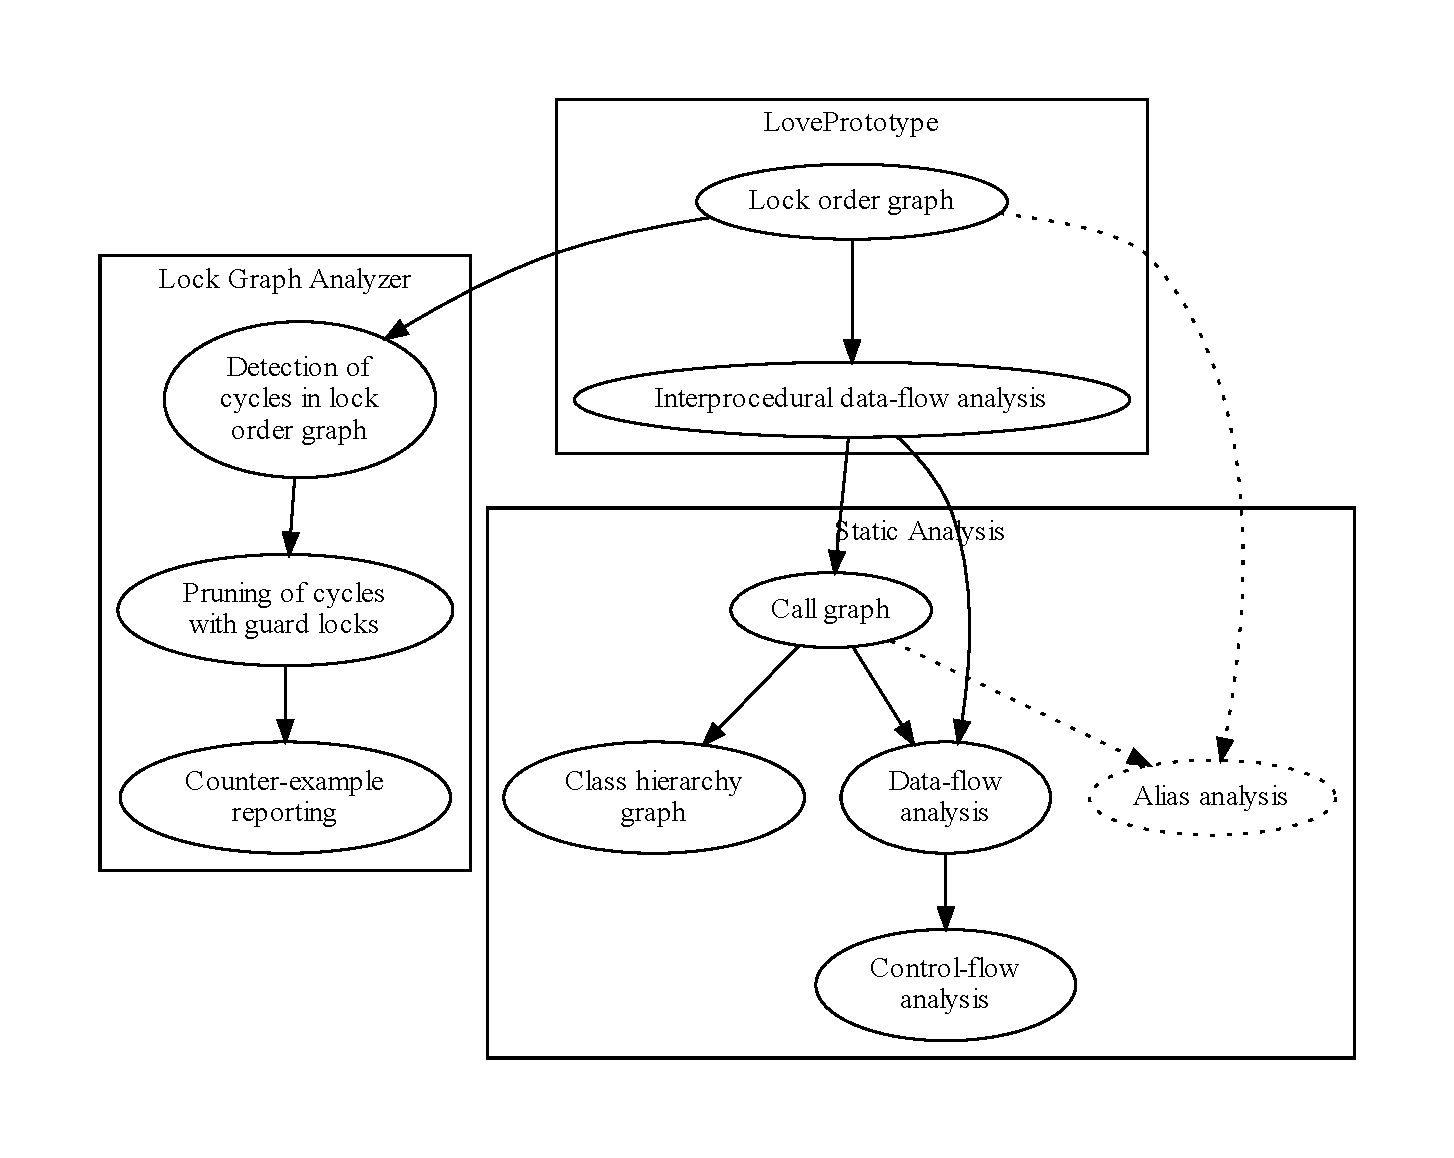
\includegraphics[scale=0.5]{Architecture.pdf}
\caption{High-level architecture of the tool}
\label{fig:architecture}
\end{center}
\end{figure}

The high-level architecture of the tool is shown on Figure ~\ref{fig:architecture}.

Mono.Cecil \citep{MonoCecil} library is used for manipulation of the program assemblies and their low-level structure and code in the intermediate language.

QuickGraph \citep{QuickGraph} library is used for manipulation of graphs. The library provides data structures for representing graphs and implements a wide variety of standard graph algorithms that operate on these data structures.

A library of common static analysis techniques is built on top of Mono.Cecil and QuickGraph libraries. It supplies a reusable implementation of class hierarchy extraction, control-flow analysis, data-flow analysis and call graph extraction.

On top of the static analysis library the \emph{LovePrototype} tool is built that constructs a call graph and then extracts the lock order graph using interprocedural data-flow analysis. The output of the tool is a lock order graph written to a file in GML (graph markup language) format.

\emph{Lock Graph Analyzer} tool is provided for analysis of the lock order graph. It takes the GML file as an input and searches the lock order graph for potential deadlocks and reports each of them into a separate DOT file. The DOT file contains the graph representing the lock order violation and accompanying information. It can be rendered using the GraphViz \citep{GraphViz} or MSAGL \citep{MsAgl} tools.

Additionally, several tools were developed to aid visualizing the graphs that are used during the analysis. Namely the \emph{GraphInspector} library, which provides a quick way of visually browsing through a graph by navigating through successors and predecessors of a highlighted vertex, and the \emph{GmlToSea} tool, which converts the standard GML format to an input suitable for the Walrus tool \citep{Walrus}.

\section{Static analysis library}

Control-flow graph can be constructed using the \texttt{ControlFlowGraph} object. The construction of the graph follows the algorithm described in Section 3. Exception flow is separated from the normal flow except for \texttt{finally} blocks, which are considered a part of the normal flow.

Data-flow analysis is implemented using a \texttt{DataFlowProblem} abstract class, which specifies the rules for data-flow analysis, such as a flow function, the initial state and the merge operator. The solution to the abstract problem can be computed using \texttt{WorkListSolver}, which takes a problem description and a control-flow graph as parameters and uses the work-list algorithm to compute the solution as either a summary state or in- and out- states for individual basic blocks. Initially, the work-list is populated with all vertices of the control-flow graph. A depth-first search is used to sort the vertices in order to minimize recomputation. Vertices that are not part any cycle are consequently sorted in topological order. The solver operates on regular vertices of the control-flow graph and doesn't traverse the exception handlers.

An abstract call graph concept is implemented. The abstraction allows switching between different call graph extraction algorithms as appropriate for the specific task without requiring a change to the call graph consumer.

A \texttt{ChaCallGraphBuilder} call graph builder implements the simple class-hierarchy based call graph extraction algorithm as described in Chapter 2. All reachable methods from a single entrypoint are analyzed and added to the call graph. Virtual method calls are resolved using the declared variable type and class hierarchy graph. Delegates are resolved by matching the delegate type. For example, each new EventHandler(FunctionX) call contributes an edge between EventHandler.Invoke and FunctionX.

\begin{figure}
\begin{center}
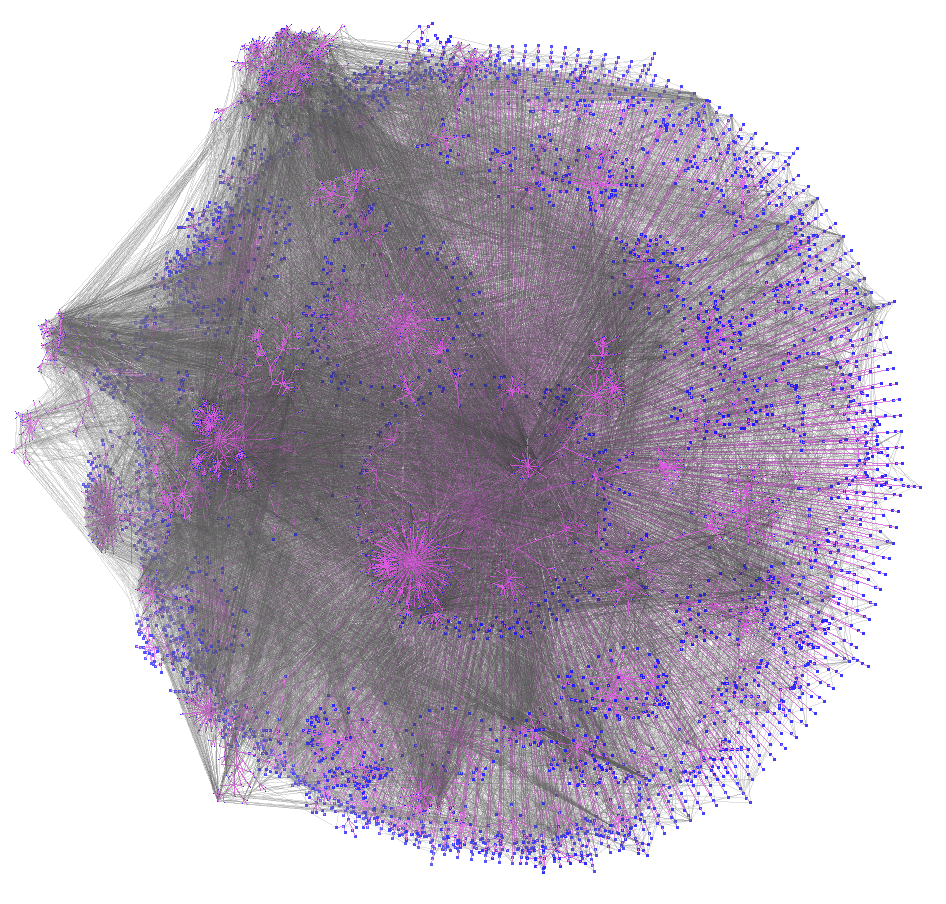
\includegraphics[scale=0.5]{CallGraph.png}
\end{center}
\caption{Computed rooted CHA call graph of a simple C\# test case program with three methods, as visualized by Walrus. The graph contains 7,177 vertices (methods) and 34,692 edges (calls), most of which come from the referenced Base Class Library. Moderately sized programs often have more than 100,000 vertices and 950,000 edges in the call graph, which is hard to visualize.}
\end{figure}

\section{LovePrototype tool}

The LovePrototype tool implements the design specified in Chapter 5. It uses the Static Analysis library for performing the intraprocedural data-flow computations and implements the interprocedural data-flow analysis using a work-list approach.

Additionally, the symbolic object aliasing behavior has several quirks that should be noted:
\begin{itemize*}
\item Fields and static fields marked as \texttt{readonly} are treated as unaliased. While this is unsound assumption it covers the most common locking pattern, where a \texttt{readonly} field is initialized with \texttt{new object()} and locked on.
\item Additional command line option \texttt{--noaliasing} is available that forces all fields to be treated as unaliased. This emulates the behavior of CSLint \citep{CSLint}.
\item Symbolic objects that represent method arguments keep reference to the original parameter they represent and thus two arguments of the same type are represented by distinct symbolic objects unlike the description in Chapter 5.
\end{itemize*} 

Command line option \texttt{--ignoresystemnamespace} is provided to suppress the analysis of all methods in the \texttt{System} namespace. This call graph is still built from all referenced classes and libraries and it is traversed even for methods belonging to the \texttt{System} namespace, locks are however not tracked.

Output of the tool is the call graph and lock graph in GML graph format with marked vertices that belong to the root set.

\begin{figure}[H]
\begin{center}
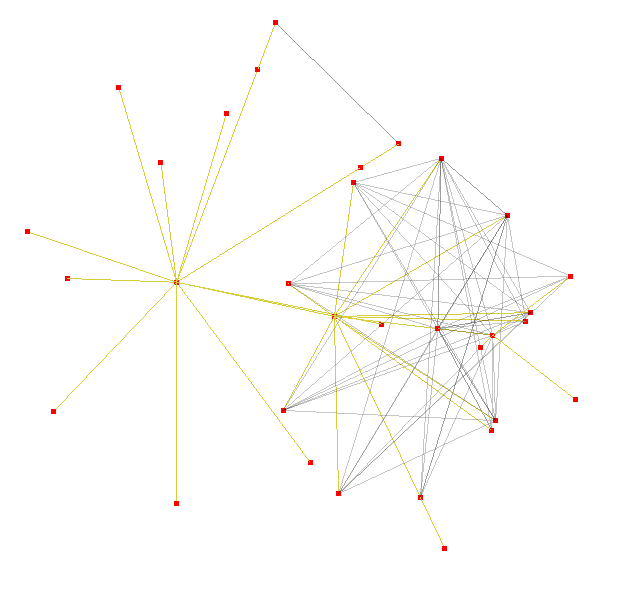
\includegraphics[scale=0.5]{LockGraph.png}
\end{center}
\caption{Computed lock graph of a simple C\# test case program with three methods, as visualized by Walrus. Tree edges are displayed in yellow and non-tree edges in gray.}
\end{figure}

\section{Lock Graph Analyzer}

The lock graph analyzer tool loads the lock order graph from the GML file produced by LovePrototype tool. It then uses depth-first search to classify all the graph edges as tree edges, back edges and forward / cross edges.

Back edges signify cycles in the graph. The tool searches specifically only for simple cycles with two edges. Thus lock order violations between more than two will not be found by this tool. These violations are rarely seen in practice and it would be trivial to extend the tool to find those cycles as well, however these cycles are often false positives caused by imprecise lock order graph construction.

Once a simple cycle is found all paths from the root locks (ie. locks that are roots of the lock order hierarchy in at least one thread) to the cycle edges are examined. These paths are built from the tree edges and forward / cross edges leading to the cycle, which implies that no other cycle is formed along these paths.

Dominance sets are computed for each vertex of the paths. If there is a common dominator between all vertices of the cycle, the dominator is considered a guard lock and the simple cycle is not considered to cause a deadlock.

Otherwise, the simple cycle is written to a DOT file for further examination by the programmer. The vertices correspond to the symbolic objects and edges are marked with the program point where the corresponding objects were acquired.

\begin{figure}
\begin{center}
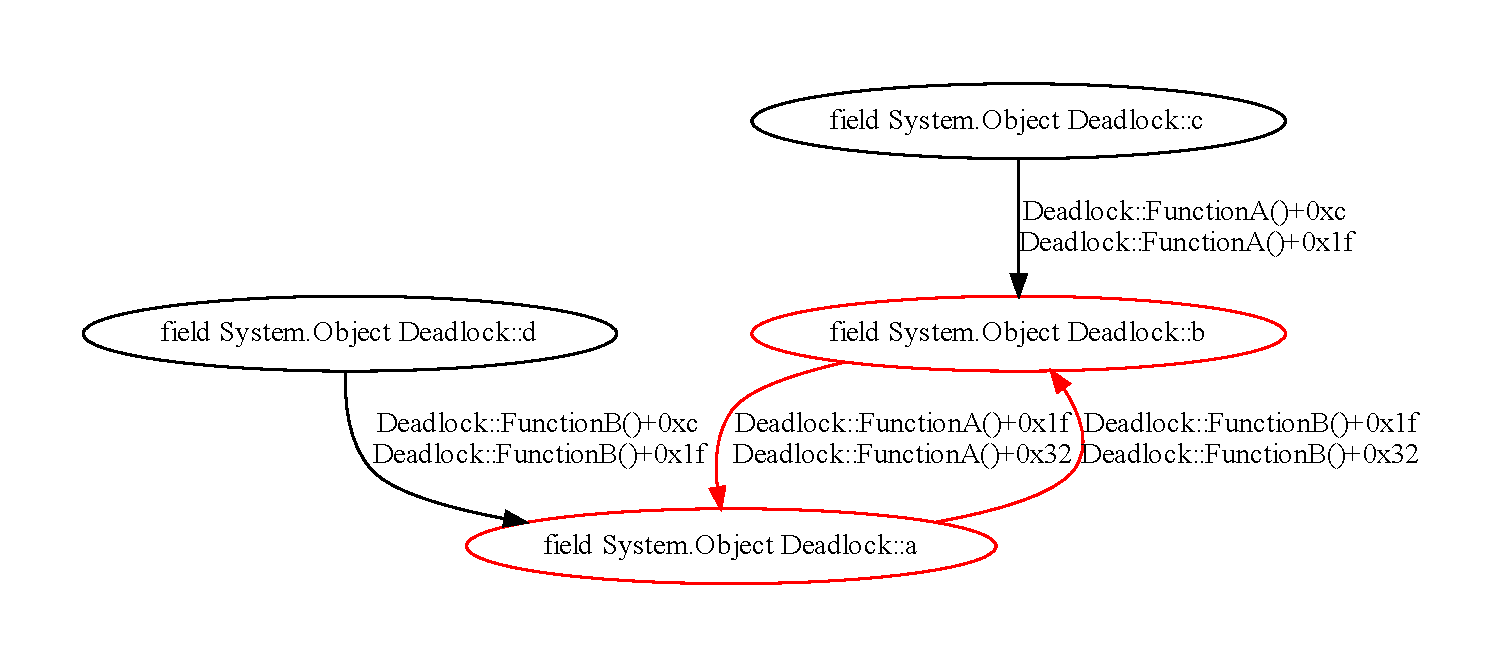
\includegraphics[scale=0.5]{LockGraphAnalyzerOutput.pdf}
\end{center}
\caption{Sample output of the Lock Graph Analyzer tool}
\end{figure}
\myepigraph{Program testing can be used to show the presence of bugs, but never to show their absence!}%
         {Edsger Dijkstra}
\chapter{Testing and experimental results}

Our benchmark consists of 12 simple test cases that cover common C\# lock patterns and one larger commercial application. The analysis was run on 1.3 GHz Intel Pentium SU4100 ULV processor with 5 GB of RAM.

\section{Test cases}

We have developed 12 simple test cases that represent the common code patterns and serve as verification for the tool:
\begin{itemize*}
\item Locking on static field (\textit{LockOnStaticField.cs})
\item Locking on instance field (\textit{LockOnField.cs})
\item Locking on \texttt{this} reference (\textit{LockOnThis.cs})
\item Locking on \texttt{typeof(Type)} (\textit{LockOnType.cs})  
\item Nested locks with no guard lock (\textit{NoGuardLock.cs})
\item Nested locks with guard lock (\textit{GuardLock.cs})
\item Thread creation using \texttt{ThreadPool.QueueUserWorkItem} (\textit{ThreadPool.cs})
\item Thread creation using \texttt{new Thread(ThreadStart f)} (\textit{Basic2.cs}) 
\item Thread creation using \texttt{new Thread(ParametrizedThreadStart f)} ( \textit{ParametrizedThreadStart.cs})
\item Nested locks across several functions (\textit{CallStack.cs})
\item Nested locks across several functions refernced by delegates (\textit{Delegate.cs})
\item Reentrancy of locks (\textit{DoubleEnter.cs}) 
\end{itemize*}
All these test cases were compiled with C\# 4.0 compiler and targeted for the .NET Framework 4.0.30319 runtime.

Additionally we use eM Client 1.0.2039 as a test case representing a larger commercial application. The code base consists of 44,928 lines of code and heavily uses multi-threading for asynchronous processing. We deliberately use an older version of the application because it was later modified to be analyzable by our unpublished CSLint fork. Additionally, most of the deadlocks present in the older version were already analyzed and are well understood, which significantly helps with the interpretation of the results.

Since we do a whole program analysis and the Base Class Library is referenced by every application, it is also implicitly included in each analysis conducted with the tool (unless the \texttt{--ignoresystemnamespace} option is used).

\section{Results}

We ran the tool with default options on the 12 simple test cases first. Analyzing each test case has taken roughly 7 seconds. The results are summarized in Figure ~\ref{fig:results01}. All expected deadlock causing patterns were identified in the test cases. Additionally 7 or 9 false positives, depending on a specific test case, are generated for the Base Class Library code. These false positives are results of impossible aliasing relationship of objects with type \texttt{System.Object}. Finally, one suspicious deadlock causing pattern (Figure ~\ref{fig:suspiciousLockingPattern}) is identified in the Base Class Library, that appears for all the test cases. The affected code is a part of .NET Remoting stack (\texttt{System.Runtime.Remoting} namespace) which is not publically exposed and thus not documented. We were unable to confirm or deny if the specific pattern can lead to a deadlock in practice or not.

% Code size, Graph size, Results
\begin{figure}[H]
\begin{center}
\begin{tabulary}{\textwidth}{ | l | r | r | r | }
\hline
Test case & \multicolumn{3}{c|}{Deadlock causing patterns} \\
\cline{2-4}
          & Reported & Confirmed & Expected\\          
\hline
Basic2 & 11 & 1 & 1 \\
CallStack & 11 & 1 & 1 \\
Delegate & 11 & 1 & 1 \\
DoubleEnter & 11 & 1 & 1 \\
GuardLock & 10 & 0 & 0 \\
LockOnField & 9 & 1 & 1 \\
LockOnStaticField & 11 & 1 & 1 \\
LockOnThis & 9 & 1 & 1 \\
LockOnType & 9 & 1 & 1 \\
NoGuardLock & 11 & 1 & 1 \\
ParametrizedThreadStart & 11 & 1 & 1 \\
ThreadPool & 9 & 1 & 1 \\
\hline
\end{tabulary}
\caption{Results for simple test cases}
\label{fig:results01}
\end{center}
\end{figure}

Next, we ran the tool with the \texttt{--ignoresystemnamespace} parameter on the same 12 simple test cases and also on eM Client. Results are summarized in Figure ~\ref{fig:results02}. For the 12 simple test cases the analysis runs in about 4 seconds and all the reports correspond to the expected deadlocks.

Analysis of eM Client took 2 minutes 40 seconds. Among the six reported deadlock patterns, only one corresponds to a real deadlock.

This deadlock pattern actually covers several possible deadlocks, which are incorrectly smeared into a single one due to overly pessimistic assumption about \texttt{System.Object} aliasing. We keep at most one edge between any two symbolic objects in the lock order graph and store the callee and caller method names along with the edge. This results in a report that isn't very intuitive for further analysis since the provided context is insufficient for throughout manual analysis.

Three other reports were caused by overly pessimistic assumption about the delegate resolution. The rest of the reports were result of a pessimistic assumptions about variable aliasing.

% Code size, Graph size, Results
\begin{figure}[H]
\begin{center}
\begin{tabulary}{\textwidth}{ | l | r | r | r | }
\hline
Test case & \multicolumn{3}{c|}{Deadlock causing patterns} \\
\cline{2-4}
          & Reported & Confirmed & Expected\\          
\hline
Basic2 & 1 & 1 & 1 \\
CallStack & 1 & 1 & 1 \\
Delegate & 1 & 1 & 1 \\
DoubleEnter & 1 & 1 & 1 \\
GuardLock & 0 & 0 & 0 \\
LockOnField & 1 & 1 & 1 \\
LockOnStaticField & 1 & 1 & 1 \\
LockOnThis & 1 & 1 & 1 \\
LockOnType & 1 & 1 & 1 \\
NoGuardLock & 1 & 1 & 1 \\
ParametrizedThreadStart & 1 & 1 & 1 \\
ThreadPool & 1 & 1 & 1 \\
eM Client & 40 & 4 & - \\
\hline
\end{tabulary}
\caption{Results for test cases when analyzed with the \texttt{--ignoresystemnamespace} parameter}
\label{fig:results02}
\end{center}
\end{figure}

Finally, we ran the tool with \texttt{--ignoresystemnamespace} and \texttt{--noaliasing} parameters. The results are summarized in Figure ~\ref{fig:results03}. For the 12 simple test cases the results were identical to previous run.

The analysis of eM Client took 2 minutes and 56 seconds and 40 reports were generated. Four of these reports were verified to be valid deadlock patterns that can actually lead to deadlock at run-time. The rest of the reports were false positives. Majority of the false positives were results of an overly pessimistic assumption about delegate resolution.

\begin{figure}[H]
\begin{center}
\begin{tabulary}{\textwidth}{ | l | r | r | r | }
\hline
Test case & \multicolumn{3}{c|}{Deadlock causing patterns} \\
\cline{2-4}
          & Reported & Confirmed & Expected\\          
\hline
Basic2 & 1 & 1 & 1 \\
CallStack & 1 & 1 & 1 \\
Delegate & 1 & 1 & 1 \\
DoubleEnter & 1 & 1 & 1 \\
GuardLock & 0 & 0 & 0 \\
LockOnField & 1 & 1 & 1 \\
LockOnStaticField & 1 & 1 & 1 \\
LockOnThis & 1 & 1 & 1 \\
LockOnType & 1 & 1 & 1 \\
NoGuardLock & 1 & 1 & 1 \\
ParametrizedThreadStart & 1 & 1 & 1 \\
ThreadPool & 1 & 1 & 1 \\
eM Client & 6 & 1 & - \\
\hline
\end{tabulary}
\caption{Results for test cases when analyzed with \texttt{--ignoresystemnamespace} and \texttt{--noalias} parameters}
\label{fig:results03}
\end{center}
\end{figure}

\begin{figure}
\begin{center}
\digraph[scale=0.45]{BCLLock}{
	rankdir="TB";
	subgraph cluster_G1
	{
		style=rounded;
		color=red;
		L1A [label = "lock(this) [Lease]", color=red];
		L2B [label = "lock(this) [Lease]",color=red];
	}
	subgraph cluster_G2
	{
		style=rounded;
		color=blue;
		L1B [label = "lock(this) [ServerIdentity]", color=blue];
		L2A [label = "lock(this.identity) [ServerIdentity]", color=blue];
	}
	"LeaseManager.LeaseTimeAnalyzer" -> "Lease.SponsorTimeout" -> "Lease.ProcessNextSponsor" -> "Lease.Cancel" -> L1A -> "RemotingServices.Disconnect" -> "IdentityHolder.RemoveIdentity" -> "ServerIdentity.ResetHandle" -> L1B;
	"..." -> "ServerIdentity.GetServerObjectChain" -> "Context.CreateServerObjectChain" -> "LeaseLifeTimeServiceProperty.GetObjectSink" -> L2A -> "Lease.Renew" -> "Lease.RenewInternal" -> L2B;
}
\caption{Suspicious locking pattern in Base Class Library}
\label{fig:suspiciousLockingPattern}
\end{center}
\end{figure}
\myepigraph{Map out your future -- but do it in pencil.}{Jon Bon Jovi}
\chapter{Future work}

\section{Improving precision}

\subsection{Alias analysis}

As we have observed, the greatest source of false positives is the lack of may-alias analysis. Adding an alias analysis would resolve two important problems -- precision of call graph and precision of symbolic objects representing fields.

Testing has shown that the very conservative over-approximation of the call graph makes the analysis not only imprecise, but also slow. The largest source of this imprecision are function pointers. As shown by \citet{Milanova2002} the FA alias analysis should be precise enough for the resolution of function pointers. 

The same alias analysis can be reused to represent symbolic objects using may-alias sets properly. It was shown by \citet{Deshmukh2009} how the basic approach we use can be extended to utilize the results of alias analysis. 

\subsection{Exception flow}

The tool we have implemented currently doesn't consider the exception handlers in the control-flow graph and thus it cannot find and lock order violation caused in the exceptional code paths.

There are two possible ways how to resolve this problem: 1) Extend the data-flow analysis solver to consider the exception handler blocks, 2) Extend the control-flow graph builder to add edges to the exception handlers.

The second approach may be easier to implement since \citet{ILSpy} have already built an implementation of the necessary code while this thesis was being written. 

\subsection{Evaluation stack}

As we have already noted in Chapter 5, the chosen model of evaluation stack is oversimplified and doesn't accurately track the indirect addresses pushed onto the stack that are later used for passing parameters by reference.

We have built the tool in a way that allows the evaluation stack model to be extended to account for other data types than the $null$ meta-symbol and references to symbolic objects.

\subsection{.override keyword}

Our implementation of the Class Hierarchy Graph doesn't account for the \texttt{.override} keyword which allows overriding method in a subclass using a different name.

This is trivial to fix, but it wasn't considered a priority since the C\# compiler can't produce intermediate code with this keyword.

\section{Extending scope}

\subsection{Lock order violation with three or more objects}

The lock analyzer tool can be extended to report simple cycles with more than two vertices, as stated in Chapter 5.

\subsection{Unbalanced Monitor.Enter and Monitor.Exit calls}

It is possible to extend the analysis to include support for unbalanced number of \texttt{Monitor.Enter} and \texttt{Monitor.Exit} calls within a single method. This could be beneficial for programs that implement custom lock types that internally use Monitor calls. % figure?

The lock state computed for each method contains the information about which locks are still held when the function returns. These locks can be aggregated into the caller's lock state when merging the callee and caller lock states. It is however possible that different targets of the call site would contribute different held locks and it is non-trivial to solve this problem.

Similarly, it would be necessary to record which locks \texttt{Monitor.Exit} was called on that were not currently held by the method. This would have to be recorded in a set in the symbolic state. When merging callee's symbolic state wiht the caller's, the locks would have to be removed from the lock state of the caller, which may once again be problematic for non-trivial cases.

\subsection{Handling of Synchronization attribute}

The \texttt{Synchronization} attribute together with the \texttt{ContextBoundObject} type provides a means for run-time interception of method calls that transparently adds synchronization around each method call. The underlying synchronization is performed using the \texttt{Monitor.Enter} and \texttt{Monitor.Exit} calls.

It it possible to extend the analysis to look for the \texttt{Synchronization} attribute and account for it when computing method summary by applying the hidden \texttt{Monitor.Enter} and \texttt{Monitor.Exit} calls to the lock state. 

%\subsection{Handling additional synchronization primitives}

%The analysis can be extended to handle additional synchronization primitives,such as those represented by WaitHandle.

% Monitor.Wait

\section{Presentation of results}

\subsection{Better counter-examples}

It would be beneficial to provide better counter-examples for the violations found by the LovePrototype tool. One possible improvement would be the inclusion of a full method call chain leading to the potential deadlock. It is possible to track this information when building the lock order graph, but it causes rapidly higher memory usage. A better approach would be to use the call graph and recompute a possible code path only when a lock order violation is found.

\subsection{Report file names and line numbers}

We currently provide method name and IL code offset in the lock order violation report. The Mono.Cecil library allows extraction of source code file name and line numbers if the accompanying debug symbols are present. It would be beneficial to use this information in the reports.
\chapter{Conclusion}

Examining programs using static code analysis requires choosing the correct static code analysis techniques and selecting a correct representation of the information we want to gather. In our case we used an interprocedural data-flow analysis on CHA call graph to compute the lock order graph. Then we extracted possible deadlock causing patterns from the lock order graph.

The current research in static program analysis of object-oriented languages is focused primarily on Java. Application of the existing principles on C\# and other .NET Framework languages was thus far limited to only handful of tools that mostly originated as a part of work in Microsoft Research.

We have developed a framework that simplifies the implementation of static program analyses on .NET code and that can serve as a basis for other research work in the area of static analysis of .NET programs.

We have further demonstrated the use of the framework for finding deadlocks in .NET programs. To our best knowledge this is the first documented implementation of interprocedural data-flow analysis of .NET code. While .NET presents more challenges than Java, such as function pointers, most off-the-shelf analyses performed on Java code could be adapted to work on .NET as well.

The experimental results obtained from the deadlock analysis tool showed that even analyzing larger programs can be done in very reasonable time. It was also shown that the tool can find actual deadlocks in a production code. The number of false positives was relatively high and we described several approaches to attack the problem that are worth pursuing in future, such as implementation of alias analysis.

While we were working on our tool and framework, another team of developers started development of the ILSpy tool \citep{ILSpy}, a decompiler and analyzer for .NET assemblies. This has resulted in the development of another static analysis library, which also works on top of the Mono.Cecil library. While the focus of this library is slightly different from ours there is some common overlap. Significant work was devoted to implementation of intermediate code representations that operate at higher level of abstraction than Common Intermediate Language. This includes abstractions similar to three-address code, SSA and abstract syntax trees. This work can play significant role when designing and implementing further static analyses of .NET code.


\bibliographystyle{abbrvnat}
\bibliography{main}

\appendix
\chapter{CD contents}

\begin{lstlisting}
Data
		Lock order graphs and call graphs presented in the
		"Testing and experimental results" chapter

Reports
		Weekly reports of the work progress

Software\NoDeadlock.Net\GmlParser
		Parser for graph markup language (GML)

Software\NoDeadlock.Net\GmlToSea
		Convertor from GML to SEA graph format

Software\NoDeadlock.Net\GraphInspector
		Library implementing GUI inspector for graphs 

Software\NoDeadlock.Net\LockGraphAnalyzer
		Tool for analyzing lock order graphs

Software\NoDeadlock.Net\LovePrototype
		Tool for generating lock order graphs from .NET
		applications

Software\NoDeadlock.Net\Mono.Cecil
		Mono.Cecil library

Software\NoDeadlock.Net\QuickGraph
		QuickGraph library

Software\NoDeadlock.Net\StaticAnalysis
		Library implementing static analysis framework

Software\Tests
		Test cases for verifying the functionality of the tools

Thesis
		Thesis text
\end{lstlisting}


\end{document}